\documentclass{beamer}

\usetheme{simple}

\usepackage{lmodern}
\usepackage[scale=2]{ccicons}
\usepackage{dirtree}

% TODO: 
%   position adjustement
%   change colours
%       

% Watermark background (simple theme)

%\setwatermark{\includegraphics[height=8cm]{img/Heckert_GNU_white.png}}


\title{}
\subtitle{STLCutter.jl}
\date{\today}
\author{Pere Antoni Martorell}
\institute{\url{http://github.com/pmartorell/STLCutters.jl}}

\begin{document}

\maketitle
\begin{frame}{Performed tests}

  Experiments from issue
  \href{https://github.com/pmartorell/STLCutters.jl/issues/11}{\#11}

  \vfill{}

  \begin{itemize}
    \item[1.1.] 
      Relative position - robustness test
      \begin{itemize}
        \item
          Set of 12 geometries
        \item
          Constant background mesh $h$-refinement% (112 divisions)
        \item
          17 relative positions ($\Delta x$ = $10^{-17:-1}$)
        \item
          17 rotation angles ($\theta$ = $10^{-17:-1}$)
      \end{itemize}
    \item[1.2.]
      Relative position - Poisson test
      \begin{itemize}
        \item
          Idem as 1.1. w/ Poisson eq. manufactured solution $u(x) = x+y-z$
      \end{itemize}
    \item[2.1.]
      $h$-refinement - robustness test
      \begin{itemize}
        \item
          1.1. geometries
        \item
          6 constant $h$-refinements
      \end{itemize}
    \item[2.2.]
      $h$-refinement - Poisson test
      \begin{itemize}
        \item
          Idem as 2.1. w/ Poisson eq. manufactured solution $u(x) = x^2+y^2-z^2$
      \end{itemize}
    \item[3.] Large geometry dataset
      \begin{itemize}
        \item   
          \href{https://ten-thousand-models.appspot.com/results.html?q=is+solid\%2C+is+manifold}
          {\underline{4963 geometries}}
          filtered from \href{https://ten-thousand-models.appspot.com}{Thingi10k}
        \item
          Unique criterion for background mesh refinement: maximum of 100 divisions per direccion
      \end{itemize}
  \end{itemize}
%  \begin{columns}[c]
%
%    \column{.45\textwidth}
%    \textbf{3. Thingi 10k dataset}
%
%    Filtered
%    \href{https://ten-thousand-models.appspot.com/results.html?q=is+closed\%2C+is+oriented\%2C+is+manifold\%2C+is+not+degenerate\%2C+without+self-intersection\%2C+\%23df\%3D0}{\underline{5k geometries}}
%    with quality criteria (closed,oriented,non degenerate...)
%
%    Tests:
%    \begin{itemize}
%      \item
%        Background mesh: 100 cells in largest direction
%      \item
%        Gadi, Titani (HPCs)
%    \end{itemize}
%    
%    
%    \column{.45\textwidth}
%    \textbf{1.1,2.1. Robustness Matrix}
%
%    Matrix axis:
%    \begin{itemize}
%      \item
%        13 geometries
%      \item
%        6 background mesh h-refinements: \texttt{14*2\^(0:5)}
%      \item
%        1 origin + 17 displacements + 17 rotation : \texttt{10\^(-17:-1)}
%    \end{itemize}
%
%  \end{columns}
\end{frame}

\begin{frame}{1.1. Relative position - Robustness test}
  \begin{block}{Setup}
    12 STLs; 17 relative positions; 17 rotation angles;  $\{\Delta x, \theta\} = 10^{-17:-1}$
  \end{block}
  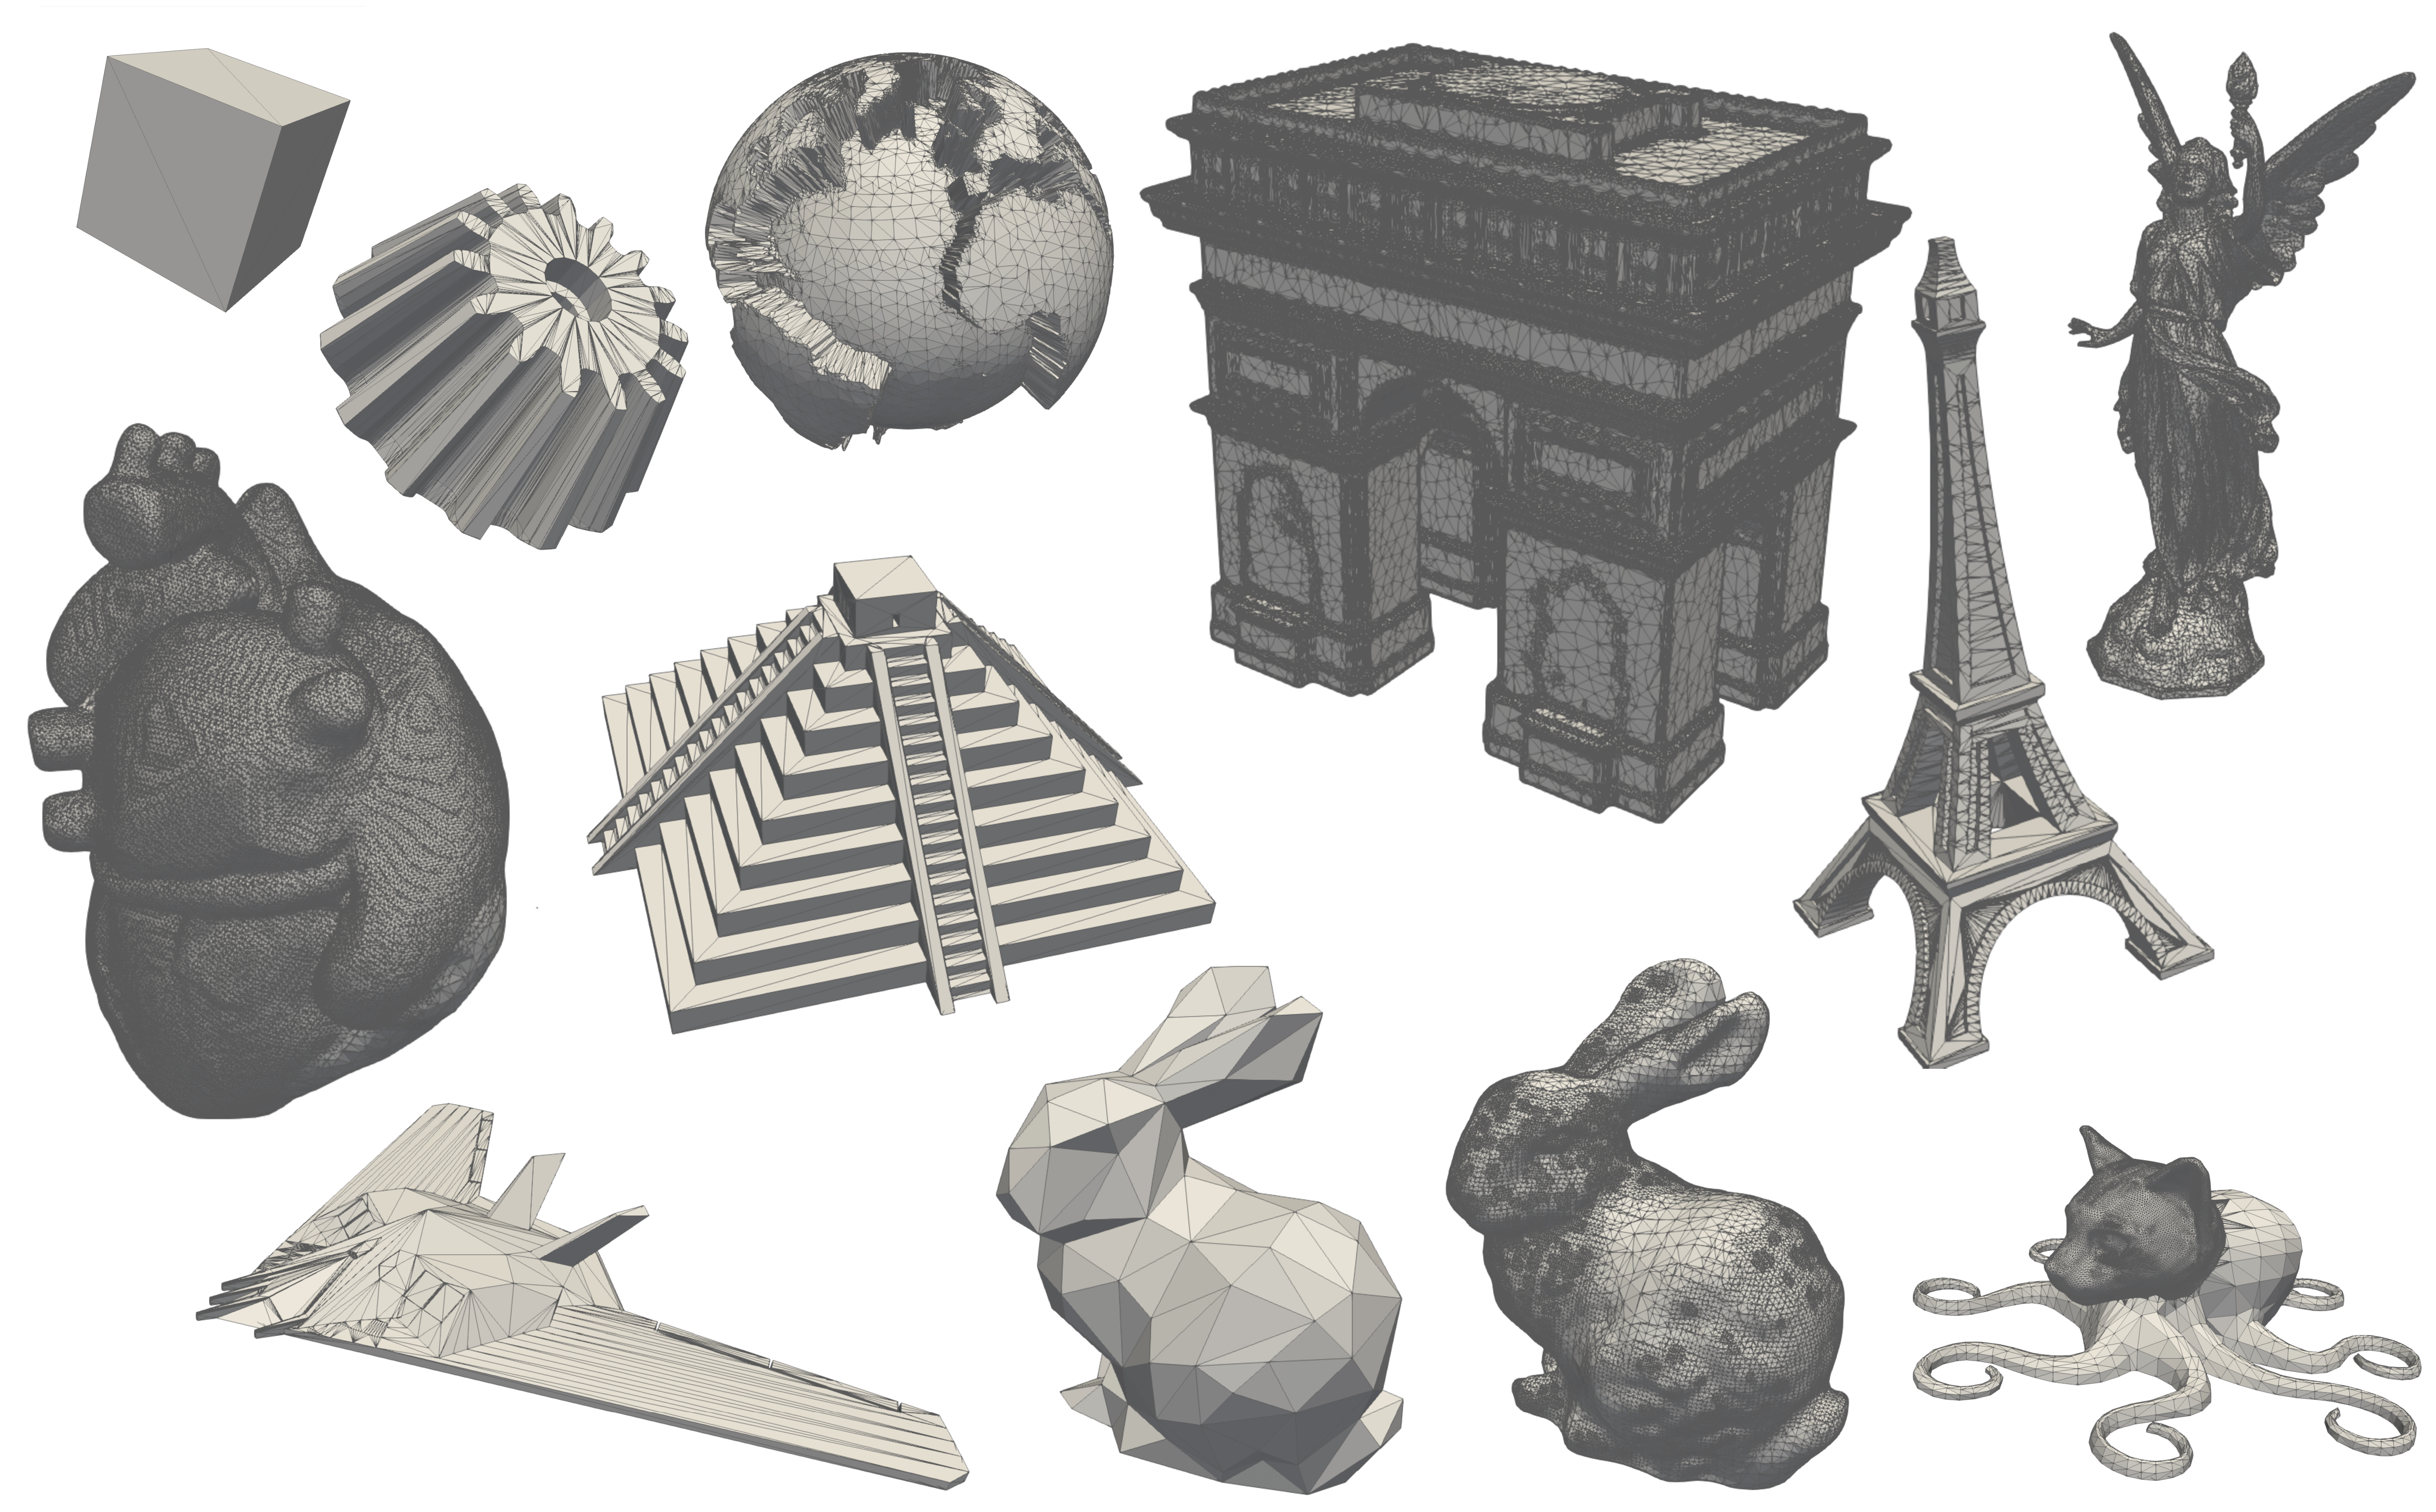
\includegraphics[width=0.95\textwidth]{matrix.pdf}
\end{frame}

\begin{frame}{1.1. Relative position - Robustness test}
  \begin{block}{Setup}
    12 STLs; 17 relative positions; 17 rotation angles;  $\{\Delta x, \theta\} = 10^{-17:-1}$
  \end{block}
  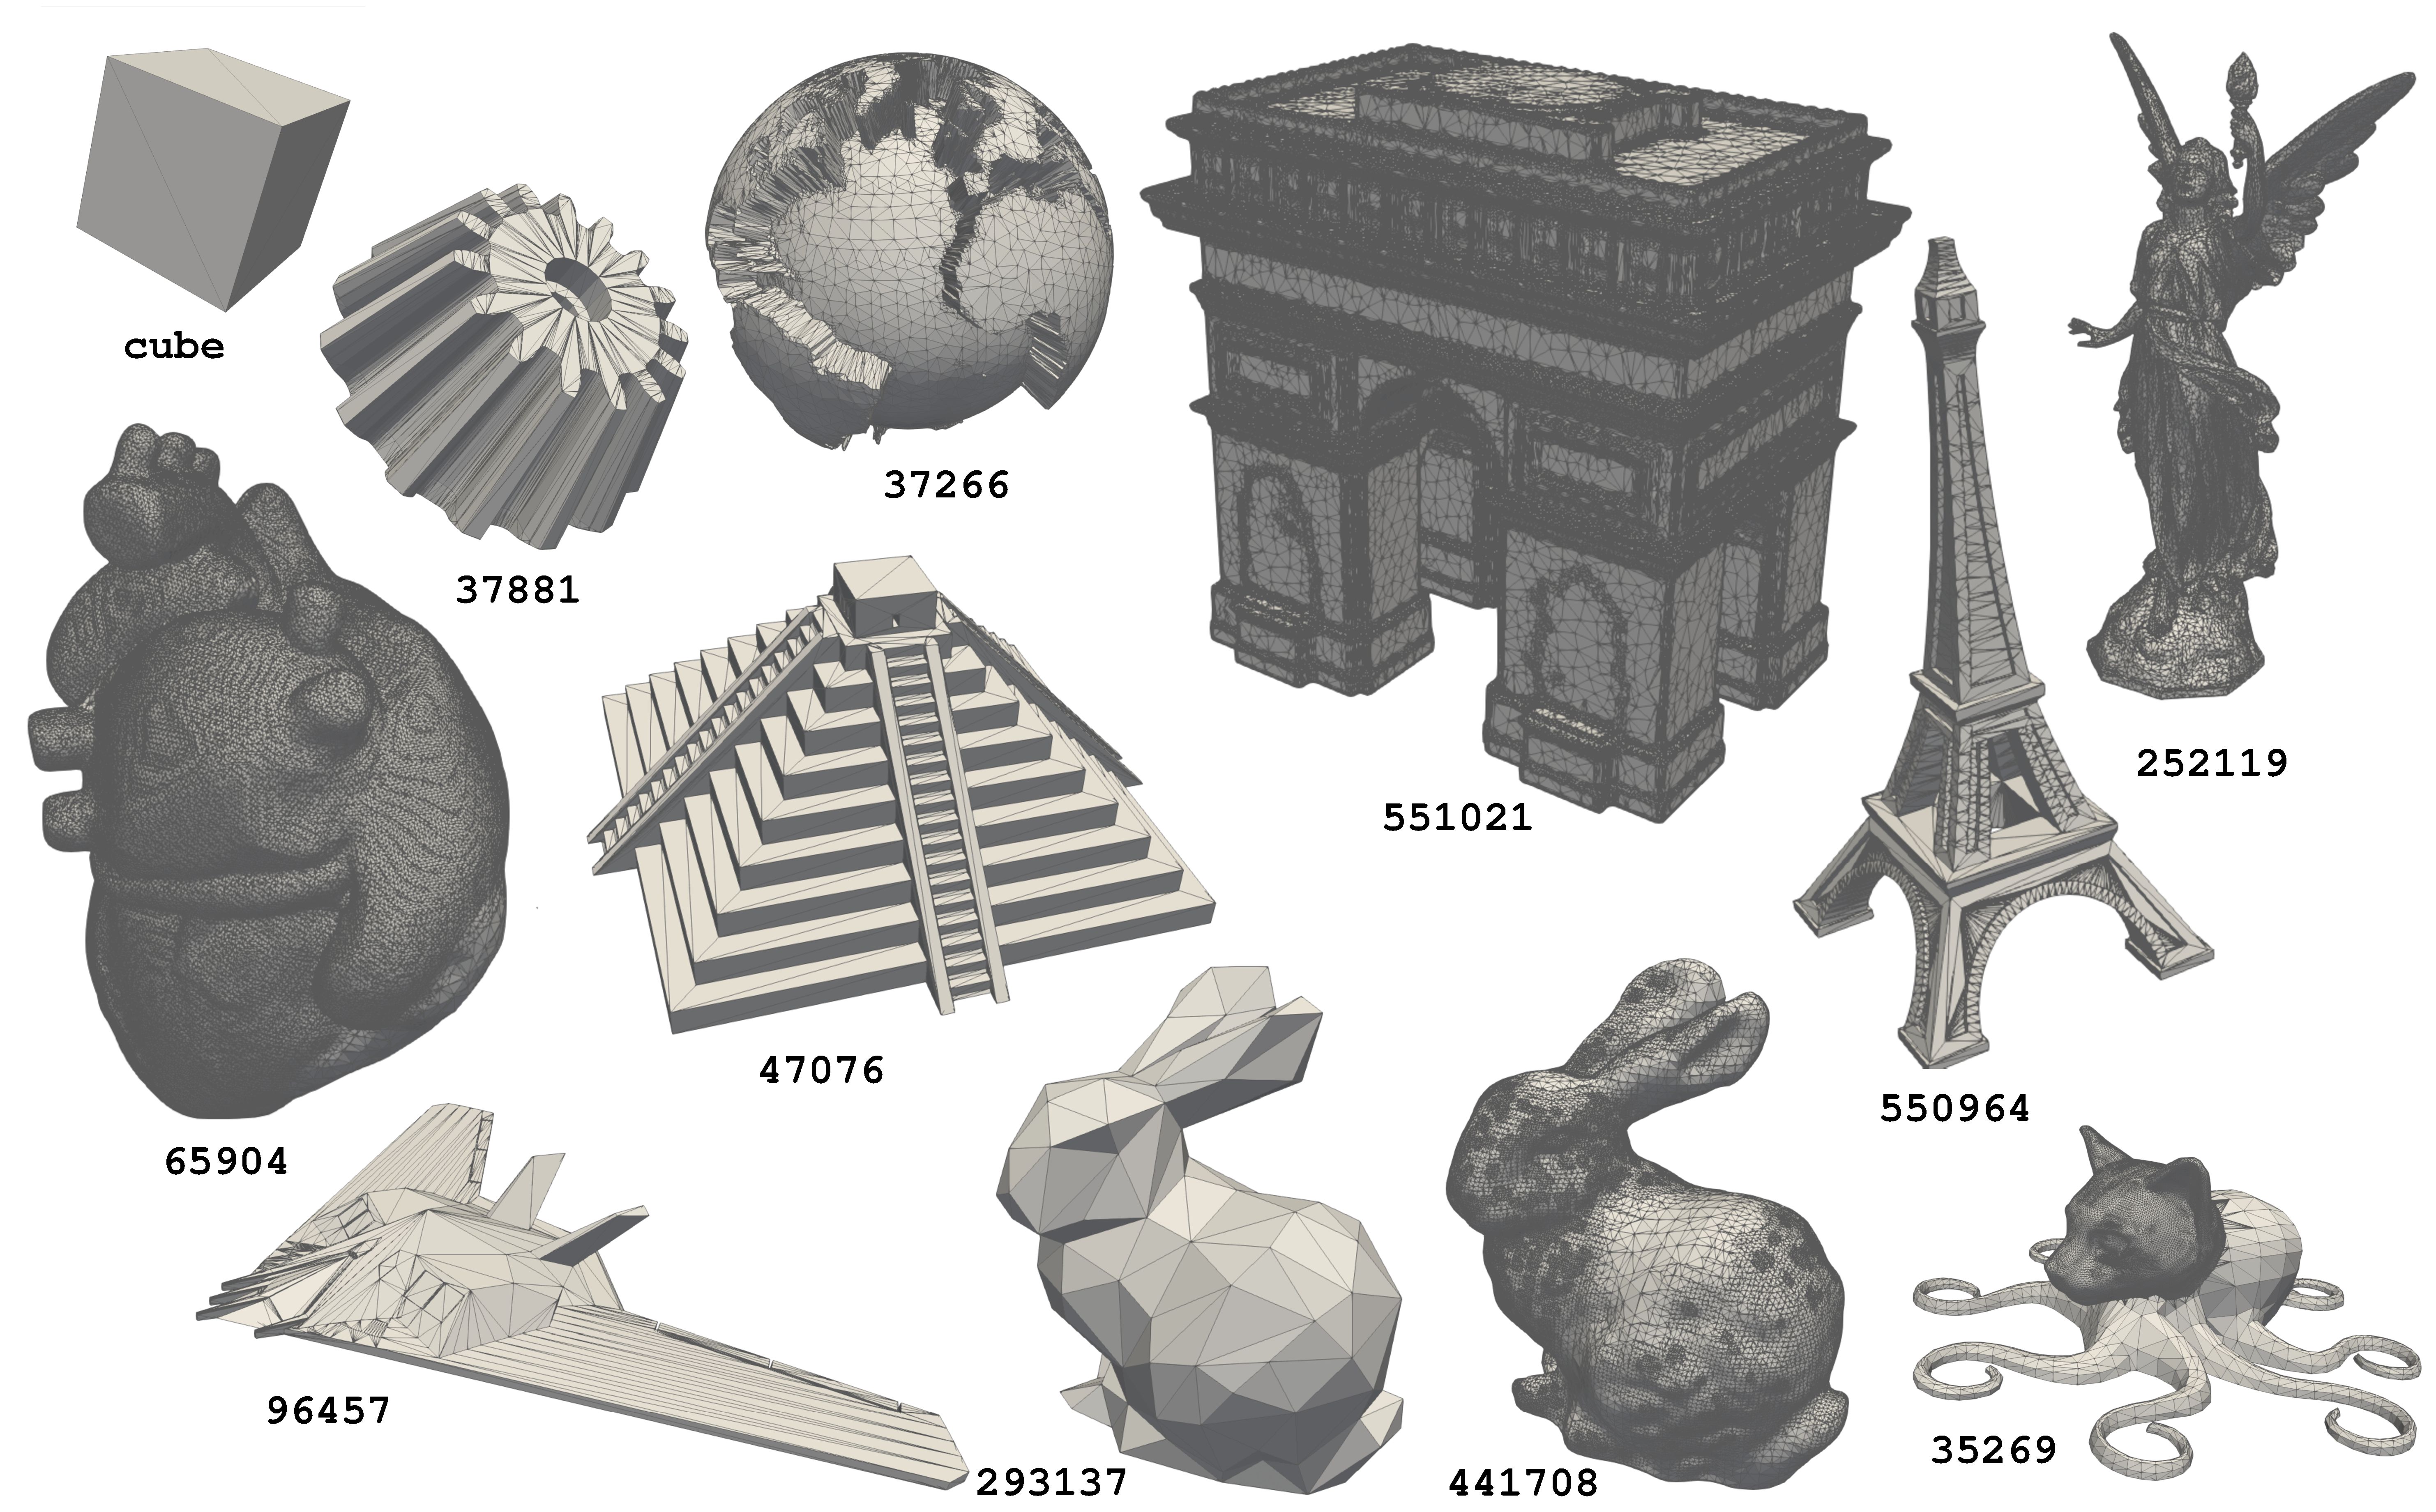
\includegraphics[width=0.95\textwidth]{matrix_ids.pdf}
\end{frame}
% thingiverse.com/download:$id
% thingiverse.com/thing:$id (wine glass)
% cube: https://people.sc.fsu.edu/~jburkardt/data/stlb/stlb.html


% Show cube ST, rotation and displacement side by side, e.g., 0,0.01,0.05,0.1

\begin{frame}{1.1. Relative position - Robustness test}

  \begin{block}{Domain volume variation}
  \begin{itemize}
    \item
      Maximum volume variation $< 10^{-14}$
  \end{itemize}
  \end{block}

  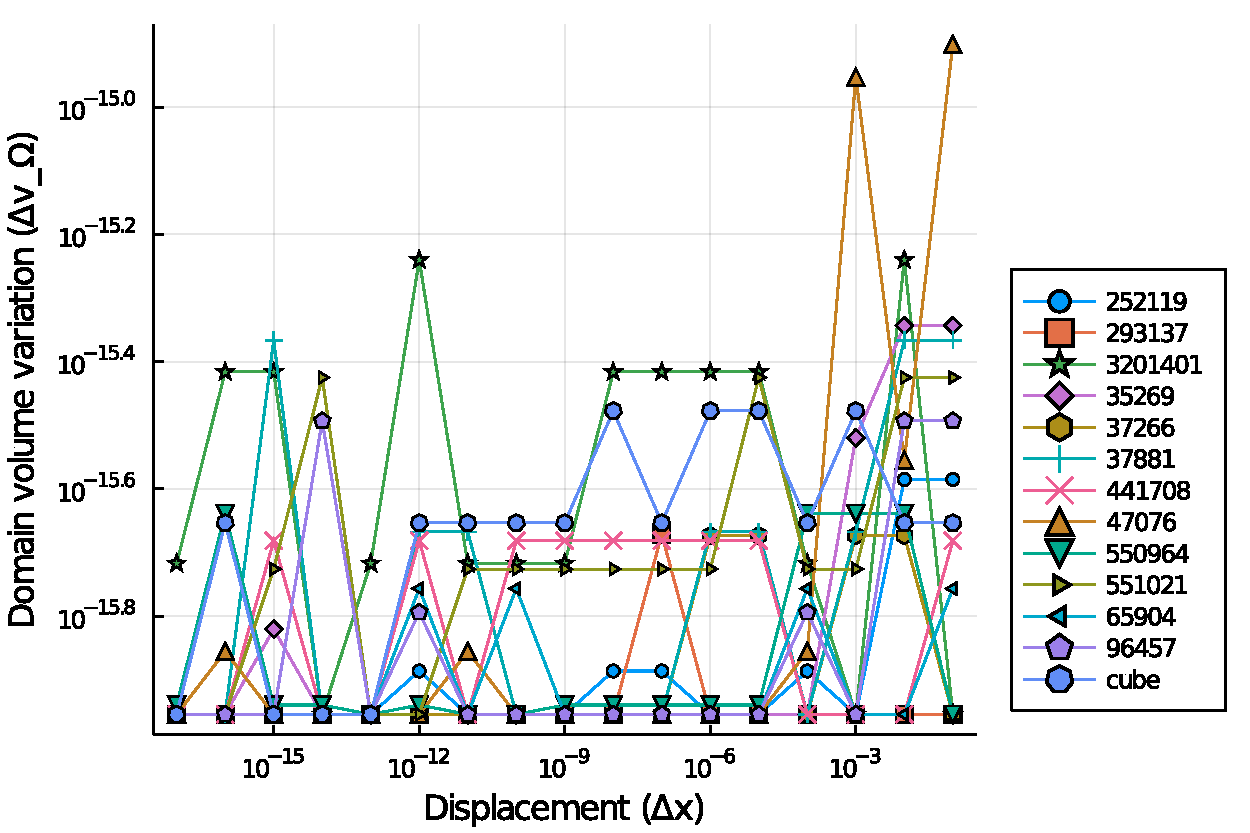
\includegraphics[width=0.49\textwidth]{../analysis/plots/x_displacement_y_domain_volume}
  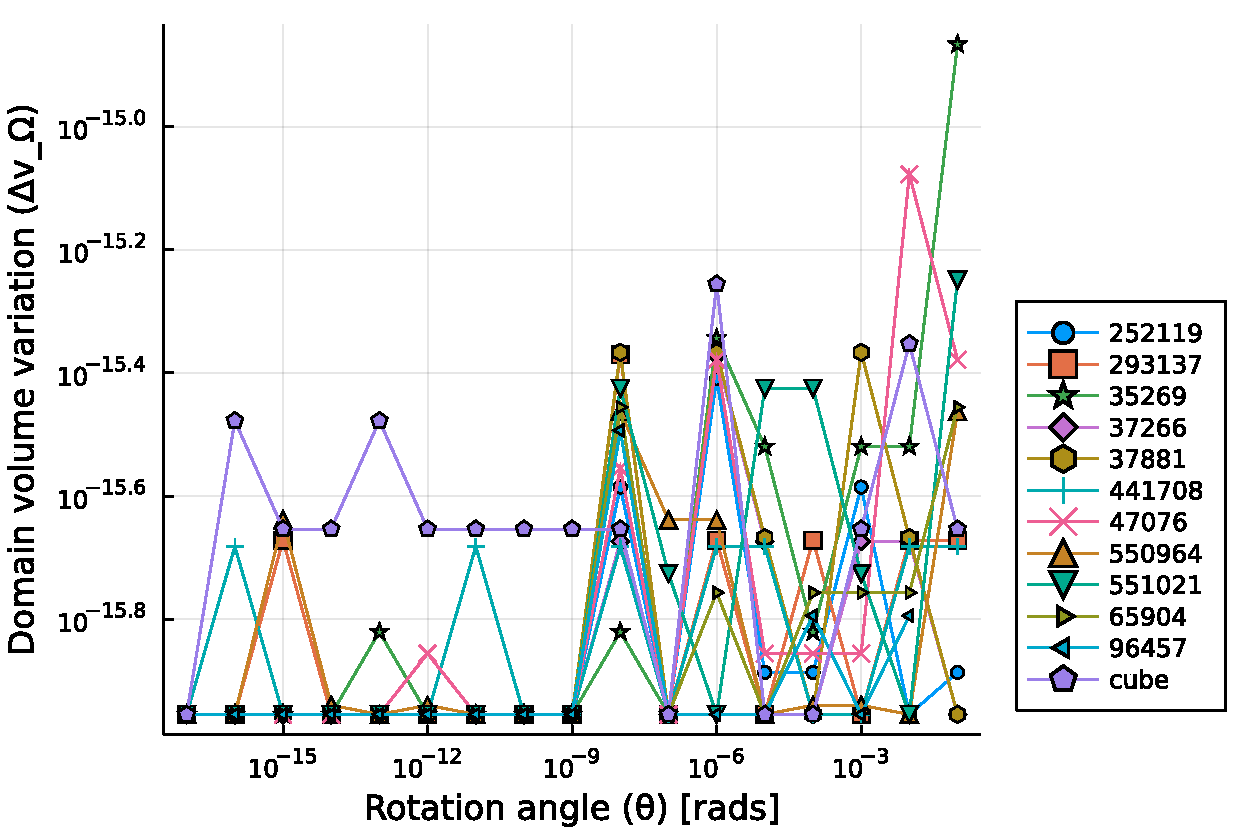
\includegraphics[width=0.49\textwidth]{../analysis/plots/x_rotation_y_domain_volume}
\end{frame}

\begin{frame}{1.1. Relative position - Robustness test}

  \begin{block}{Domain volume variation}
  \begin{itemize}
    \item
      Maximum volume variation $< 10^{-11}$
    \item
      Rotations introduce more rounding errors at planes
  \end{itemize}
  \end{block}

  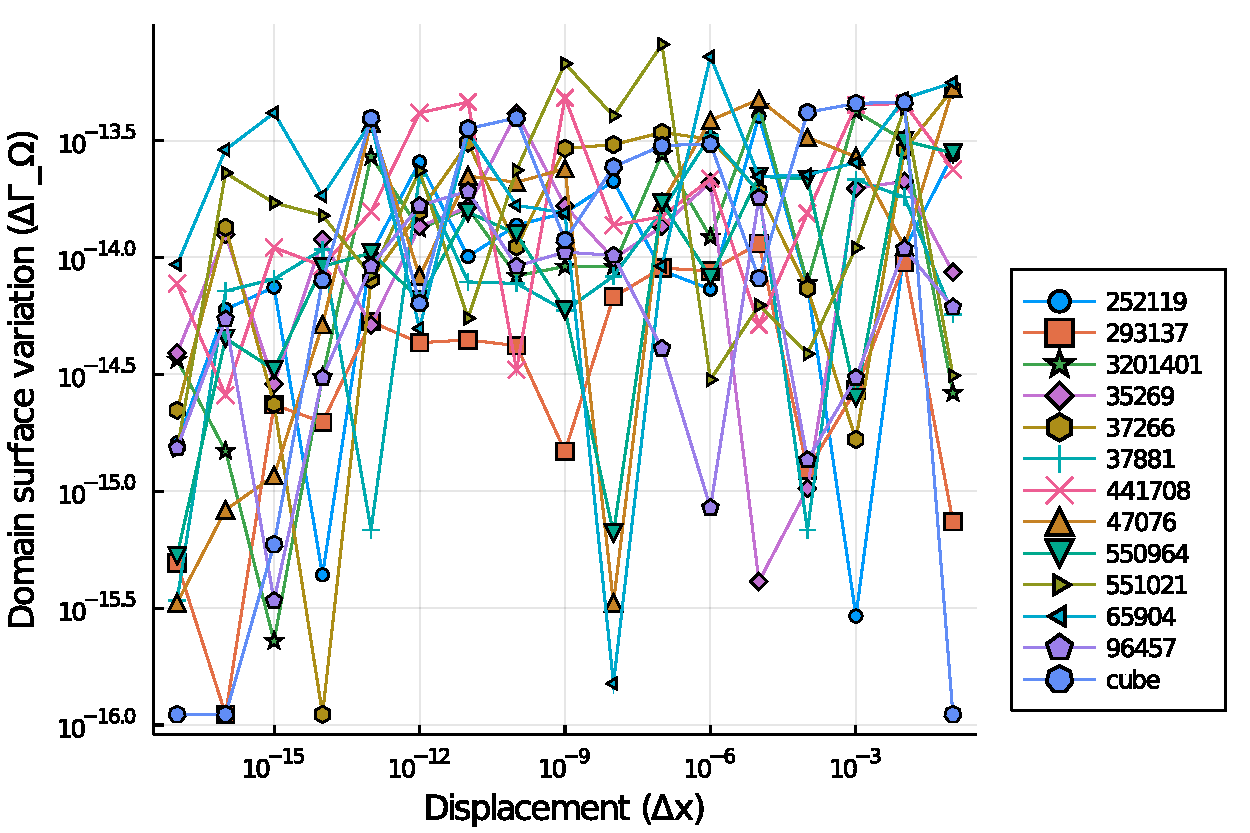
\includegraphics[width=0.49\textwidth]{../analysis/plots/x_displacement_y_domain_surface}
  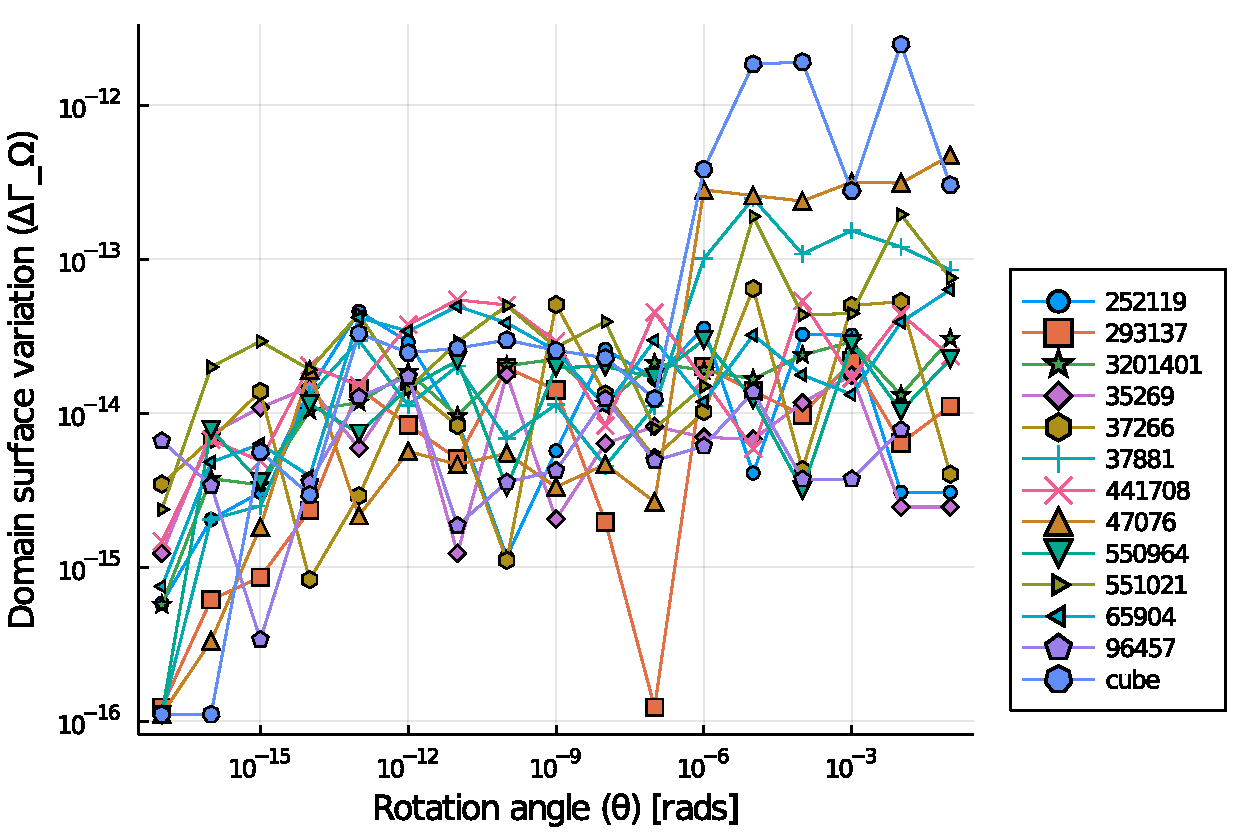
\includegraphics[width=0.49\textwidth]{../analysis/plots/x_rotation_y_domain_surface}
\end{frame}


\begin{frame}{1.2. Relative position - Poisson test}

  \begin{columns}
\column{0.5\textwidth}

  \begin{block}{Setup}
    \begin{itemize}
      \item
        Same configurations as 1.1.
      \item
        Poisson eq. w/ manufactured solution
        \begin{align*}
          -\Delta u &= f,\\
          u(x) &= x+y-z
        \end{align*}
      \item
        AgFEM w/ aggregate threshold 0.5
    \end{itemize}
  \end{block}
  
\column{0.5\textwidth}
  \centering
  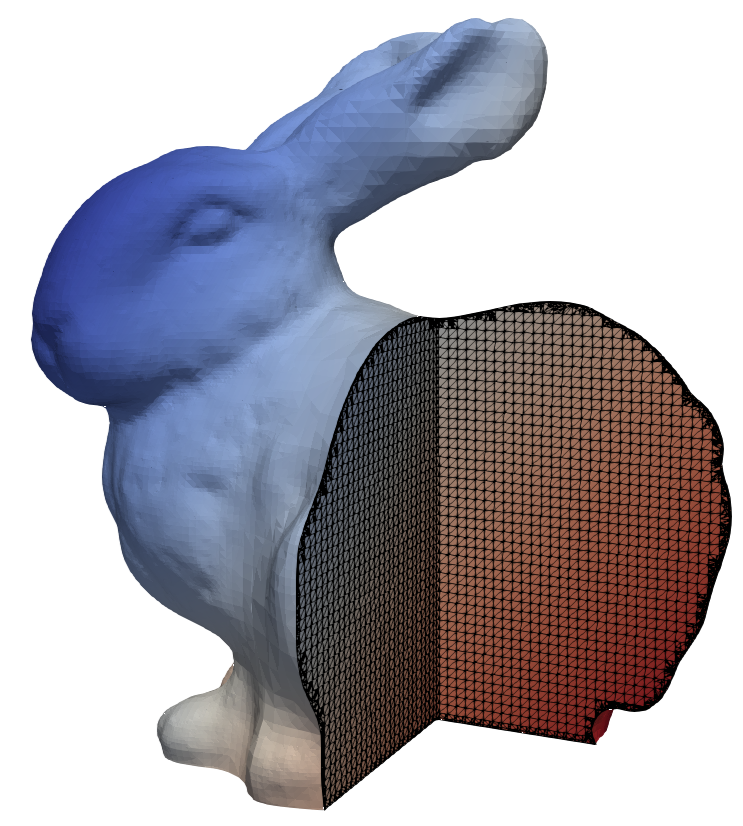
\includegraphics[width=\textwidth]{bunny_poisson_cut}
%  % add image of poisson e.g. bunny / heart when fixed
  \end{columns}
\end{frame}

\begin{frame}{1.2. Relative position - Poisson test}

  \begin{block}{H1 error norm}
  \begin{itemize}
    \item
      Maximum H1 error norm $< 10^{-12}$
    \item
      Minor variations on rotation/displacement
  \end{itemize}
  \end{block}

  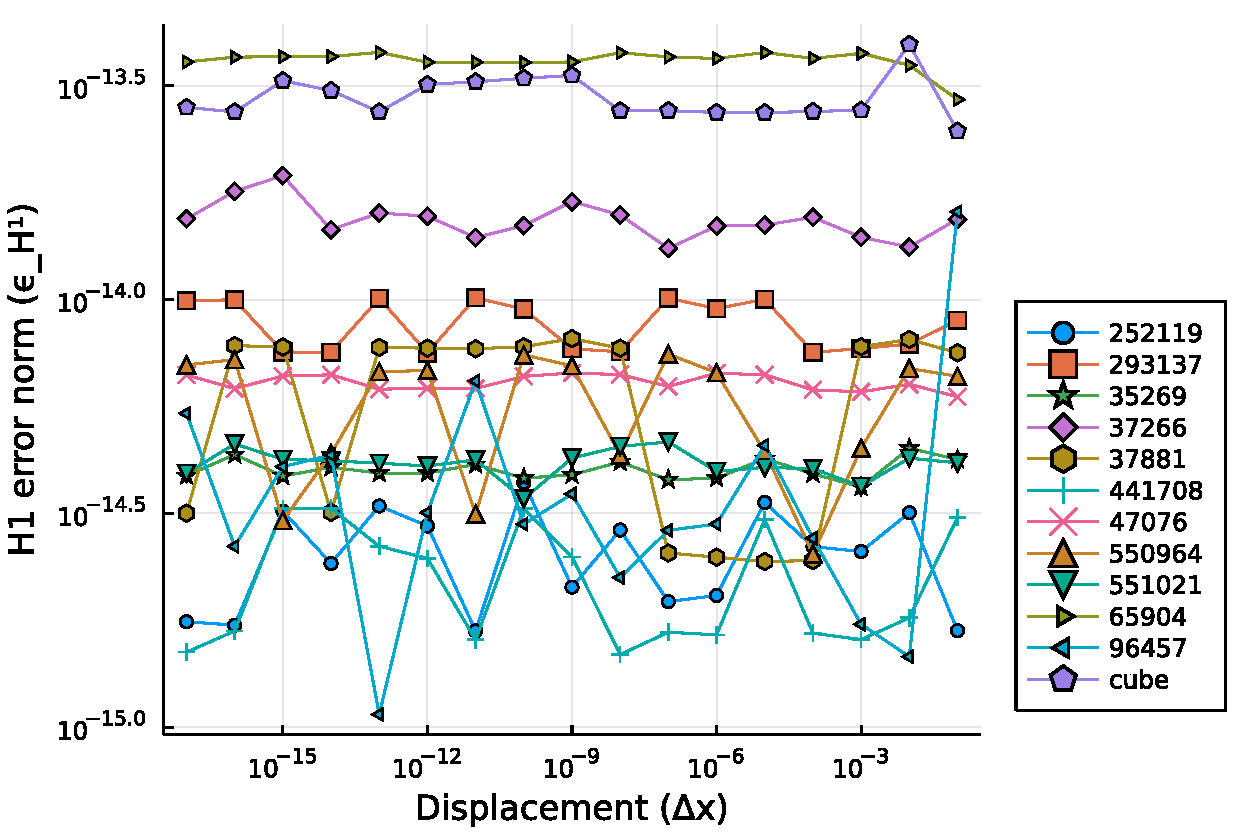
\includegraphics[width=0.49\textwidth]{../analysis/plots/x_displacement_y_error_h1}
  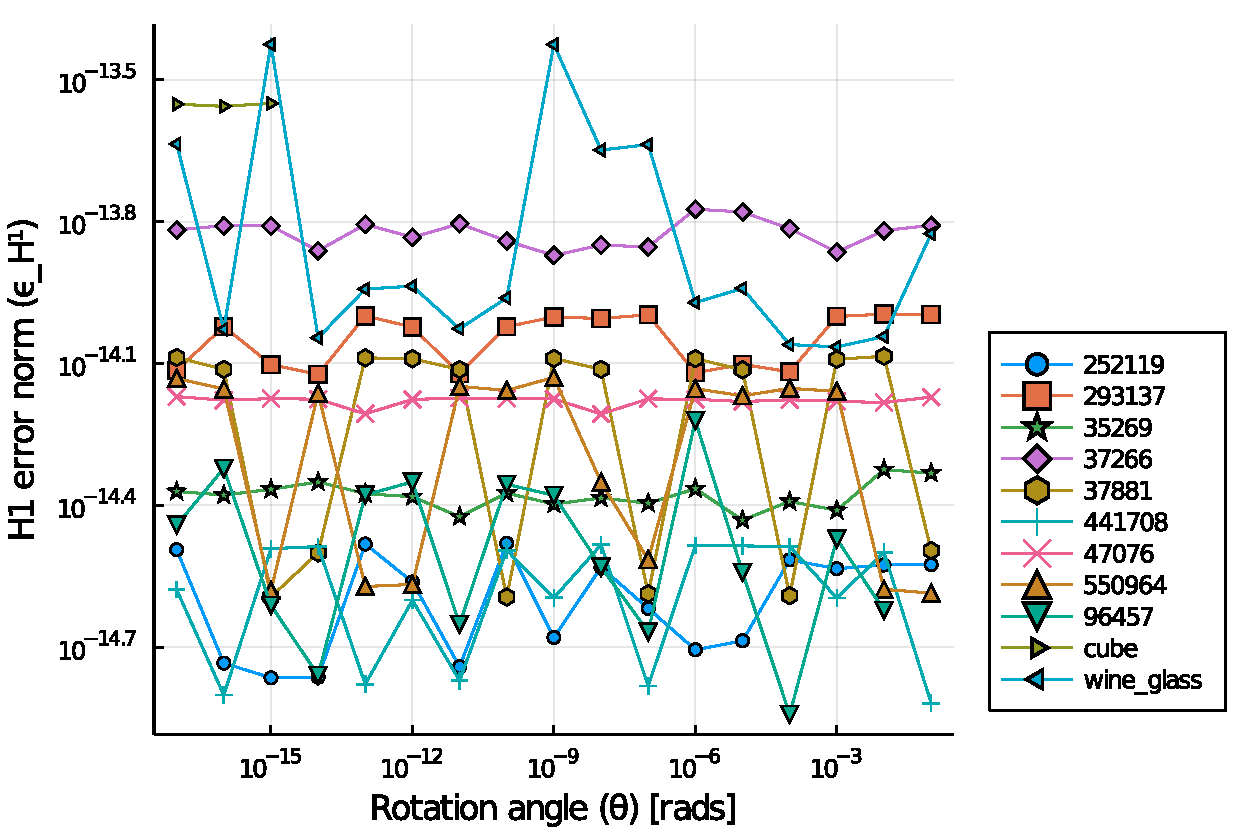
\includegraphics[width=0.49\textwidth]{../analysis/plots/x_rotation_y_error_h1}
\end{frame}

\begin{frame}{1.2. Relative position - Poisson test}

  \begin{block}{L2 error norm}
  \begin{itemize}
    \item
      Maximum L2 error norm $< 10^{-13}$
    \item
      Minor variations on rotation/displacement
  \end{itemize}
  \end{block}

  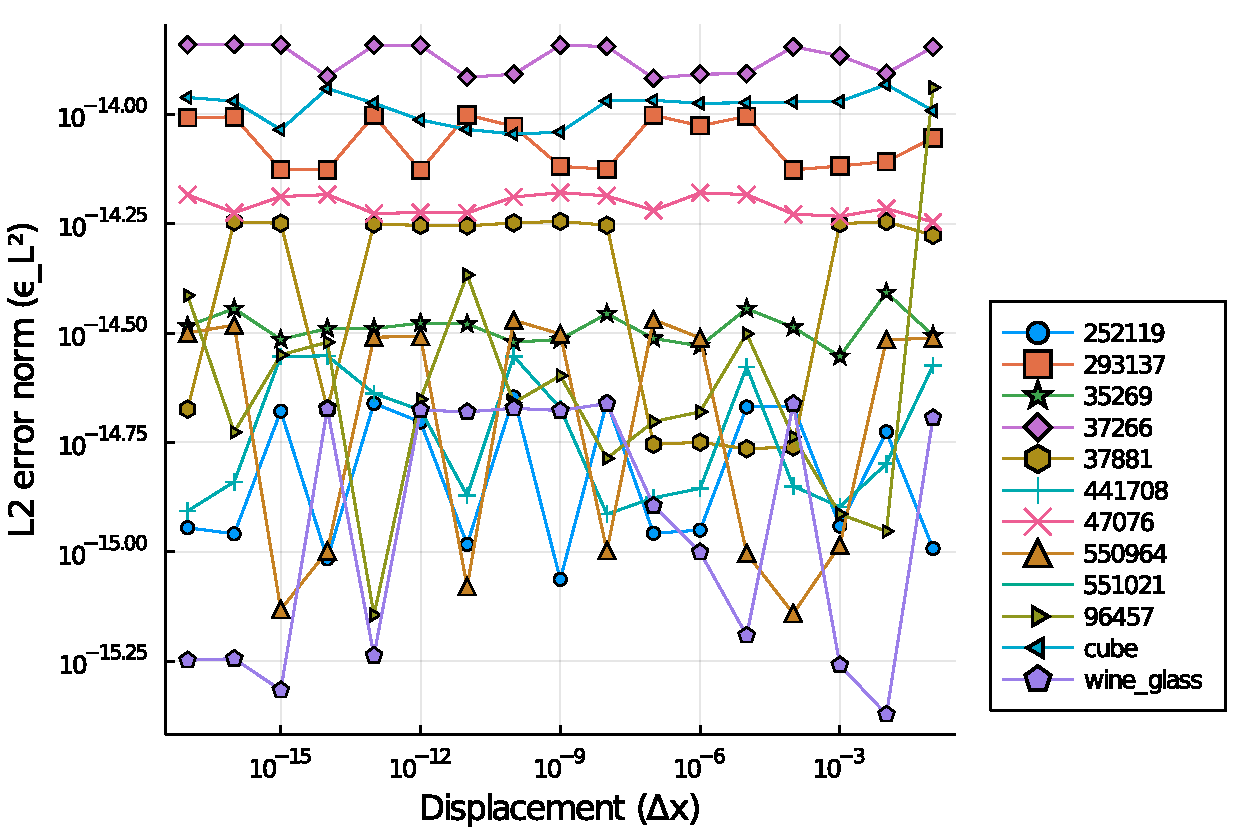
\includegraphics[width=0.49\textwidth]{../analysis/plots/x_displacement_y_error_l2}
  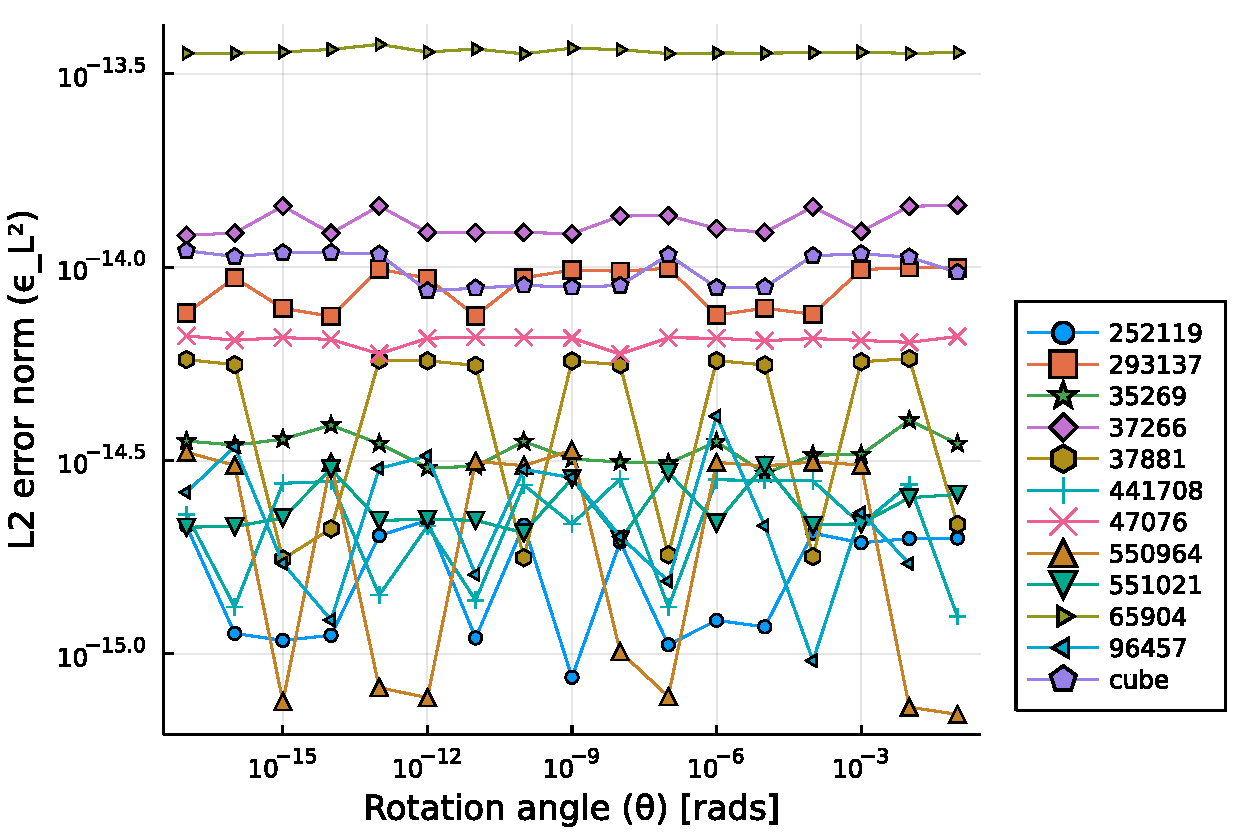
\includegraphics[width=0.49\textwidth]{../analysis/plots/x_rotation_y_error_l2}
\end{frame}


\begin{frame}{2.1. $h$-refinement - Robustness test}
  \begin{block}{Setup}
    \begin{itemize}
      \item
        12 geometries from 1.1.
      \item
        6 refinement sizes: $N_{max} = 14 \cdot 2^{0:5}$
    \end{itemize}
  \end{block}

  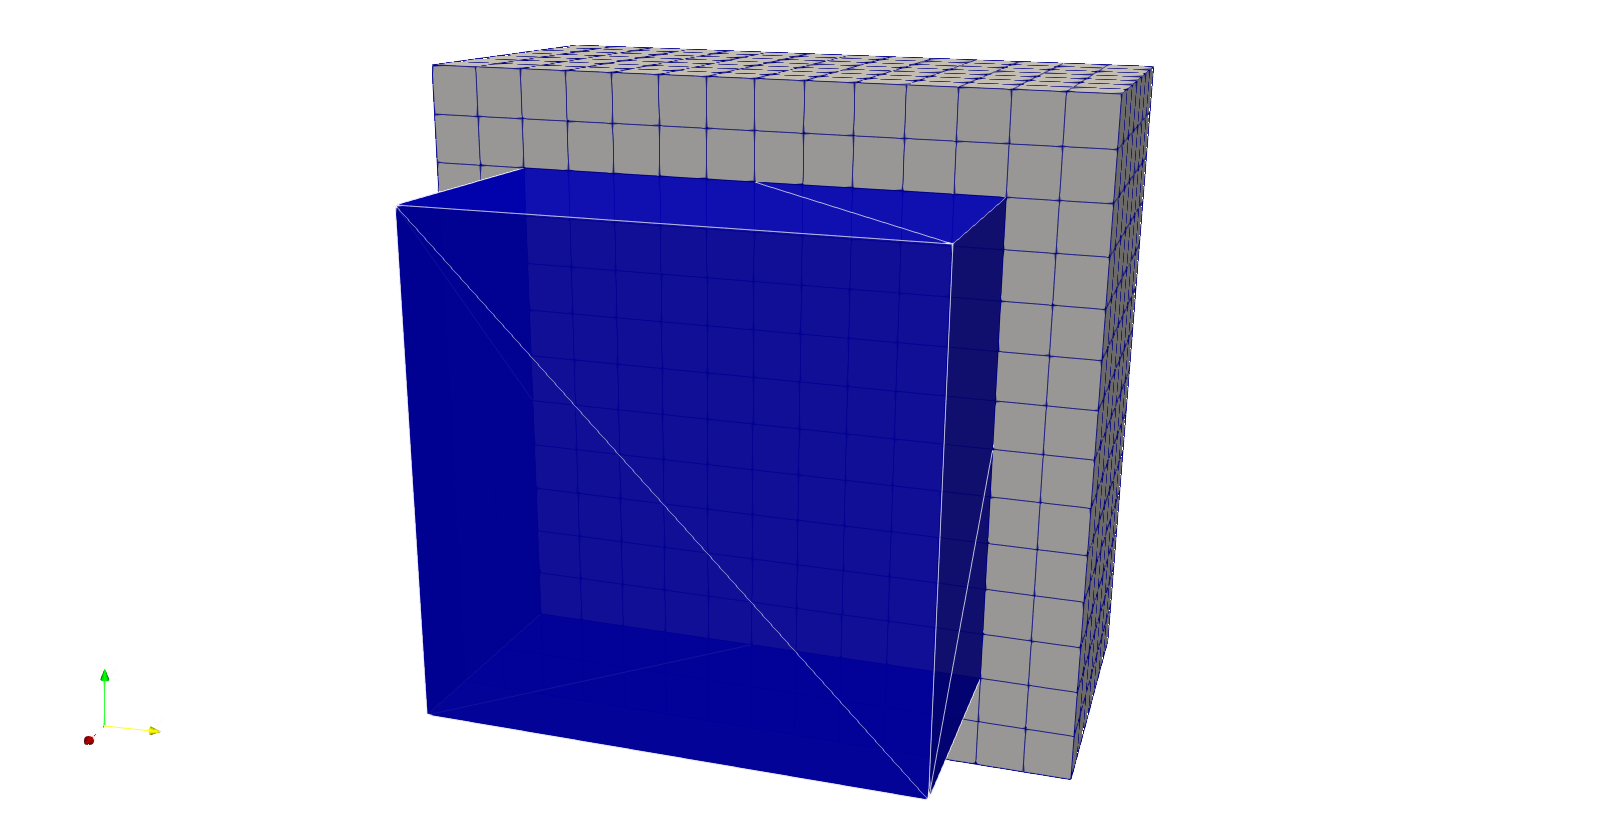
\includegraphics[width=0.7\textwidth]{cube_bb}

  \textbf{NOTE 1:} The $N_{max}$ is multiple of 14 to force the STL faces and background cell faces to be aligned, thus stress more the algorithm. As the background mesh is expanded 0.2 in each direction of the STL's bounding box.
\end{frame}

\begin{frame}{2.1. $h$-refinement - Robustness test}
  \begin{block}{Setup}
    \begin{itemize}
      \item
        12 geometries from 1.1.
      \item
        6 refinement sizes: $N_{max} = 14 \cdot 2^{0:5}$
    \end{itemize}
  \end{block}

  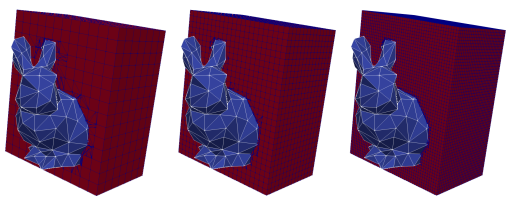
\includegraphics[width=0.95\textwidth]{h_low_bunny}

 \textbf{NOTE 2:} In order to keep the background cell aspect ratio, $N_{max}$ is the number of divisions on the largest side of the bounding box.
\end{frame}


\begin{frame}{2.1. $h$-refinement - Robustness test}

  \begin{block}{$h$-refinement}
  \begin{itemize}
    \item
      Surface variation increases with $1/h$ ($\Delta \Gamma < 10^{-11}$)
    \item
      Volume is constant at refinement ($\Delta V < 10^{-14}$)
  \end{itemize}
  \end{block}

  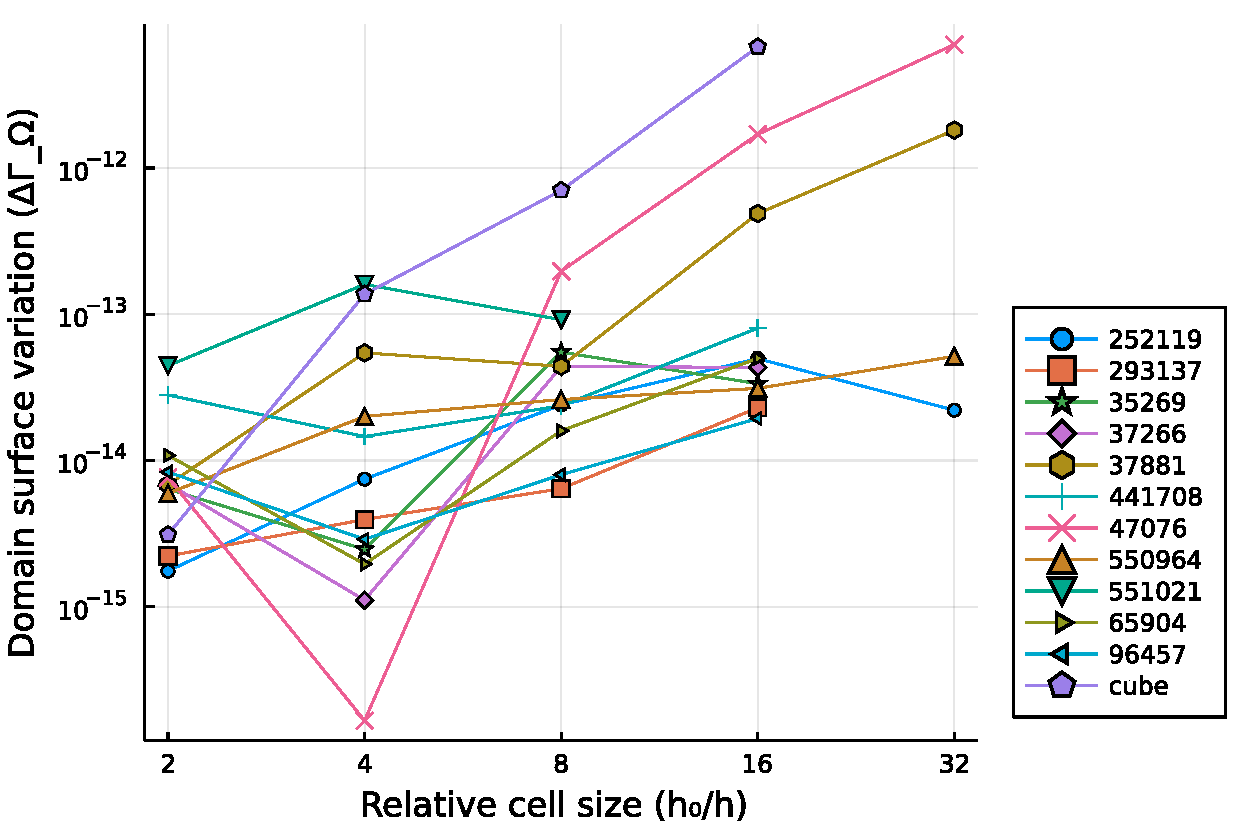
\includegraphics[width=0.49\textwidth]{../analysis/plots/x_nmax_y_domain_surface}
  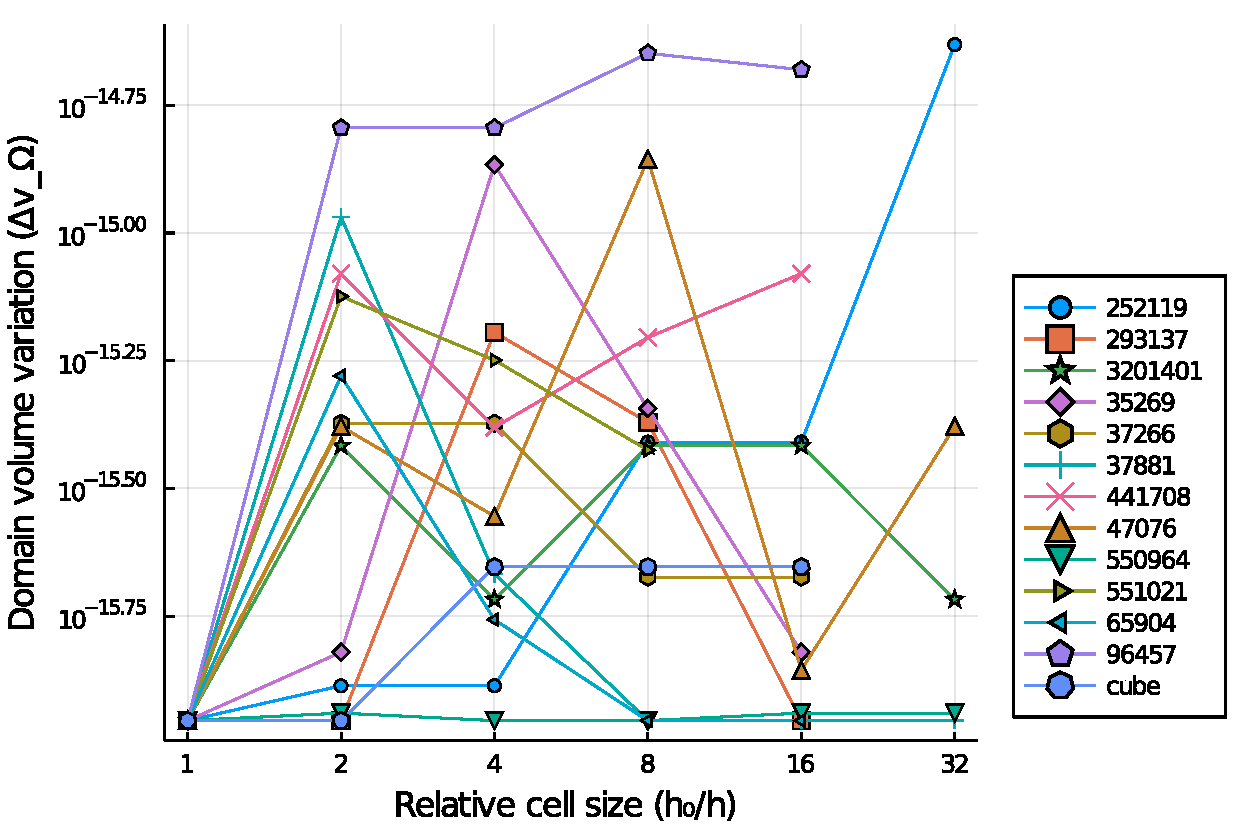
\includegraphics[width=0.49\textwidth]{../analysis/plots/x_nmax_y_domain_volume}
\end{frame}

\begin{frame}{2.1. $h$-refinement - Robustness test}

  \begin{block}{CPU time with $h$-refinement}
  \begin{itemize}
    \item
      Not precise measure (single runs)
    \item
      Tend to be linear after first complexity reduction
  \end{itemize}
  \end{block}

  \centering
  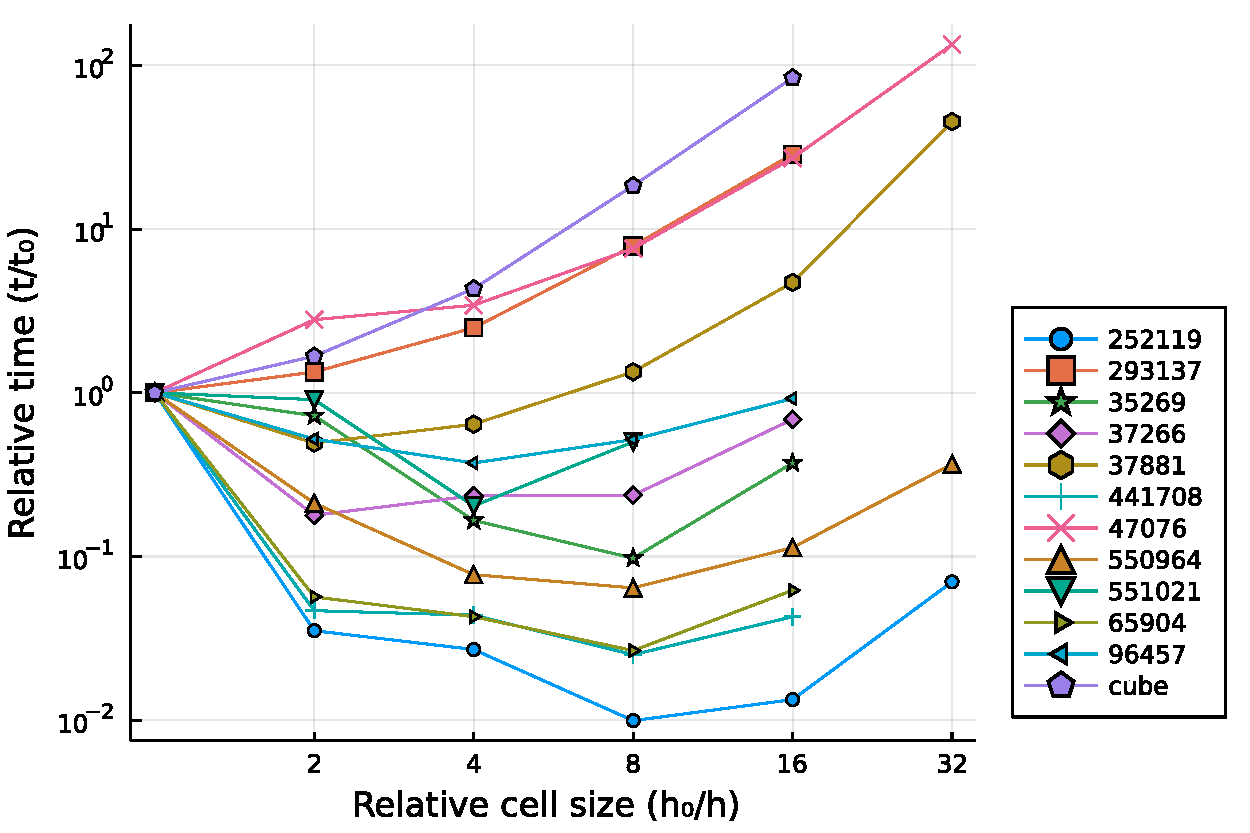
\includegraphics[width=0.60\textwidth]{../analysis/plots/x_nmax_y_time}

\end{frame}

\begin{frame}{2.2. $h$-refinement - Poisson test}
  \begin{block}{Setup}
    \begin{itemize}
      \item
        Same configurations as 2.1.
      \item
        Poisson eq. w/ manufactured solution
        \begin{align*}
          -\Delta u &= f,\\
          u(x) &= x^2+y^2-z^2
        \end{align*}
      \item
        AgFEM w/ aggregate threshold 0.5
    \end{itemize}
  \end{block}
%  \centering
%  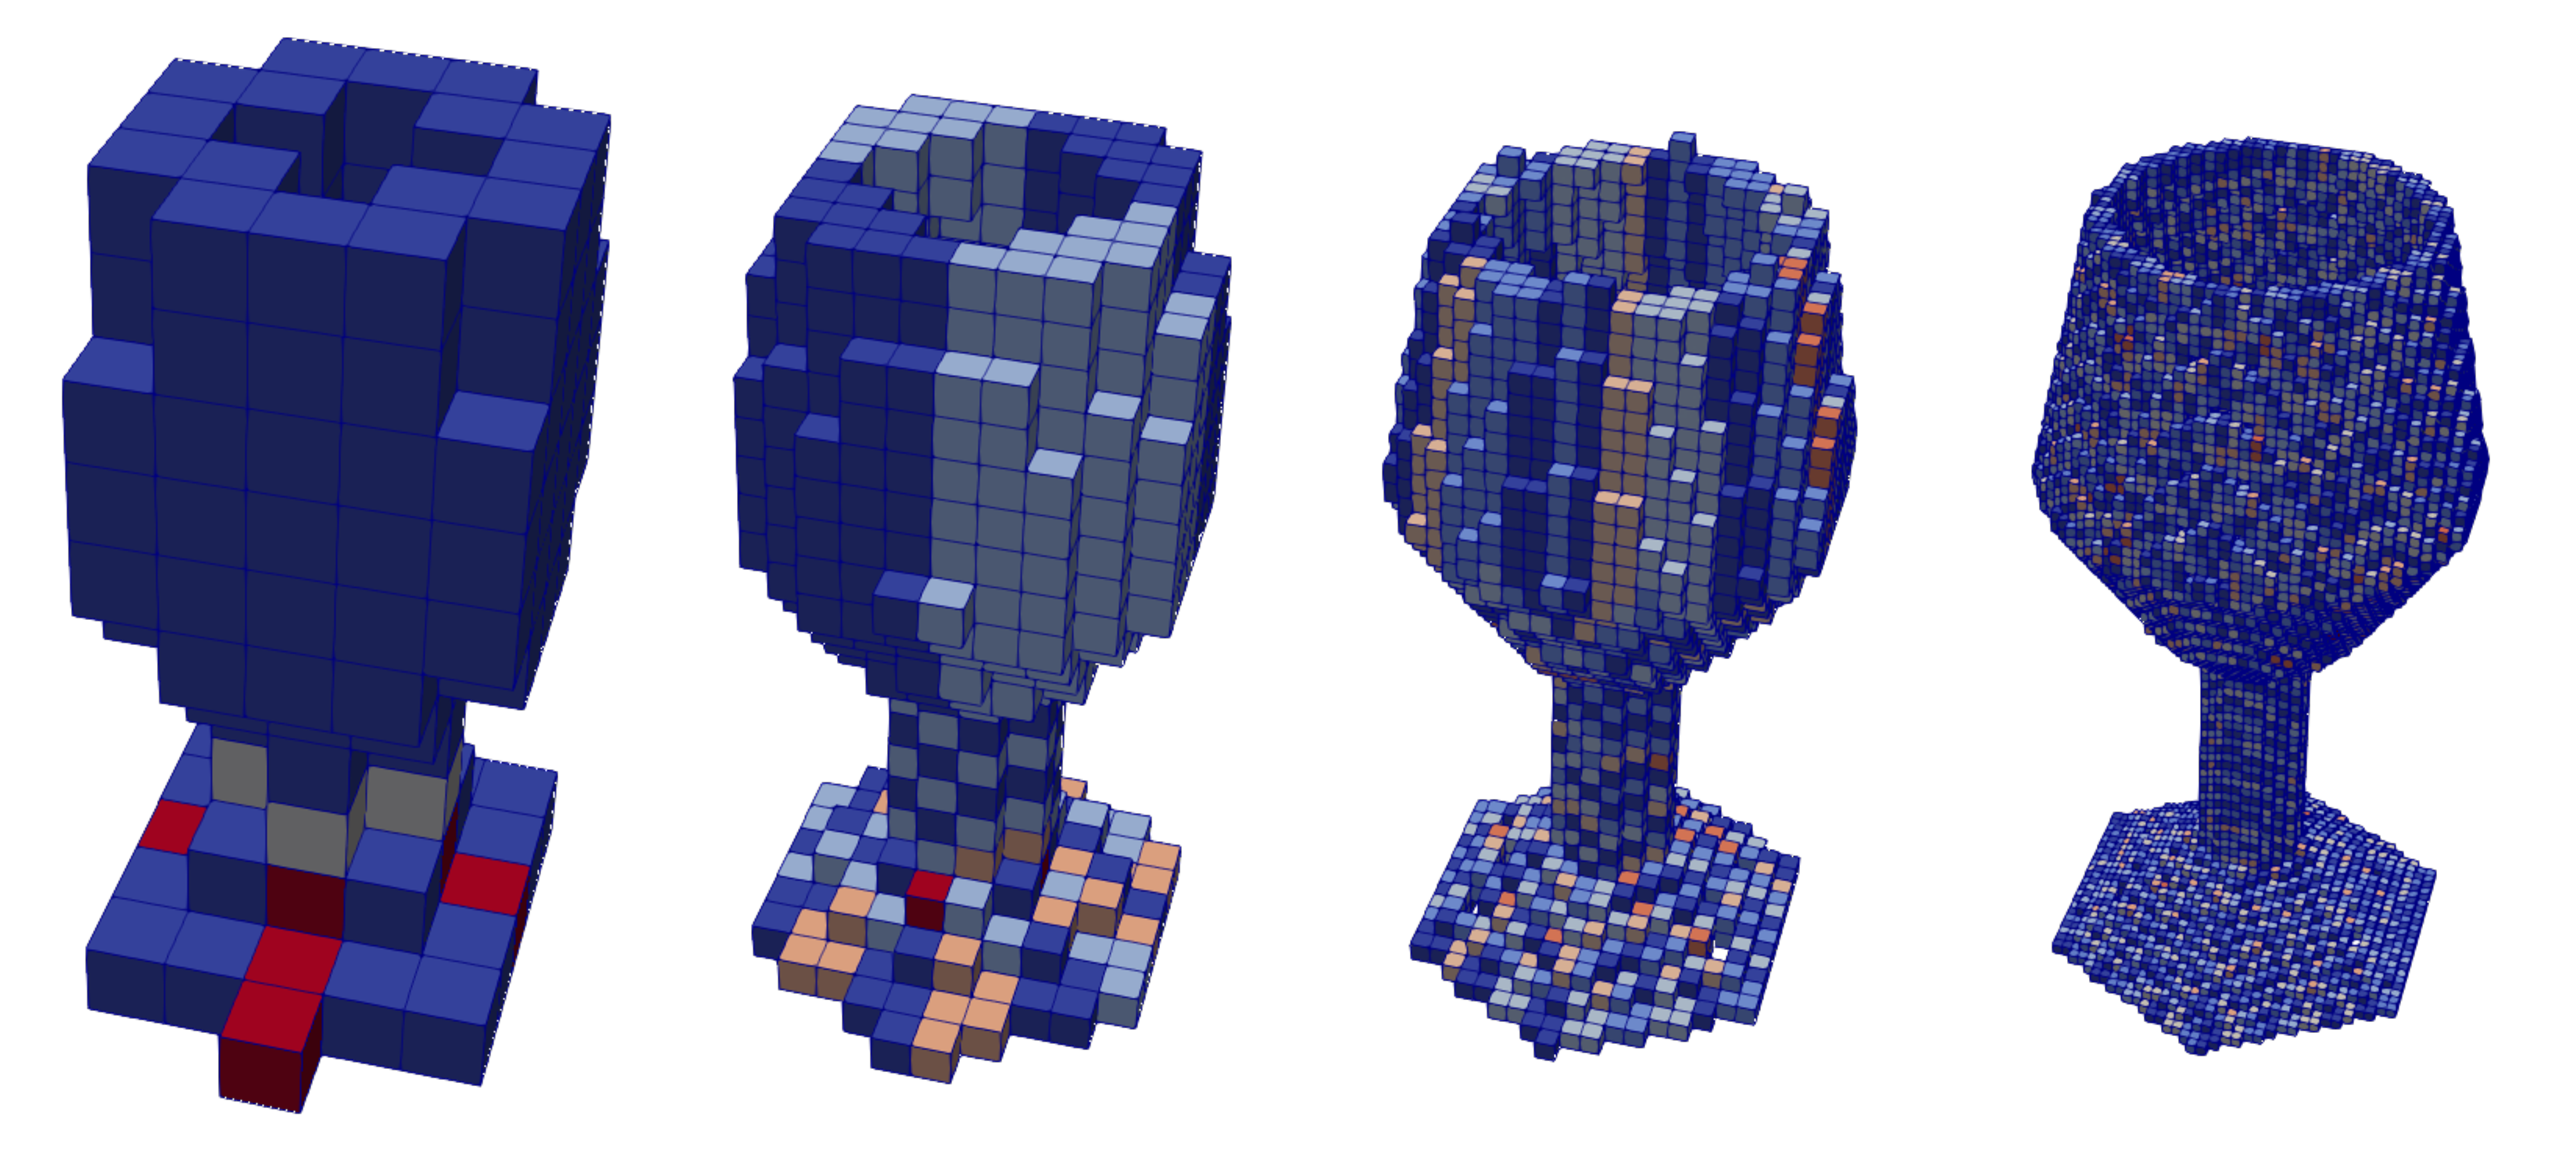
\includegraphics[width=0.7\textwidth]{aggregates}
%
%  {\tiny Cell aggregation in thin walls}

\end{frame}


\begin{frame}{2.2. $h$-refinement - Poisson test}
  \begin{block}{FE convergence with $h$}
  \begin{itemize}
    \item
      H1 and L2 error norms tend to the convergence slope
  \end{itemize}
  \end{block}

  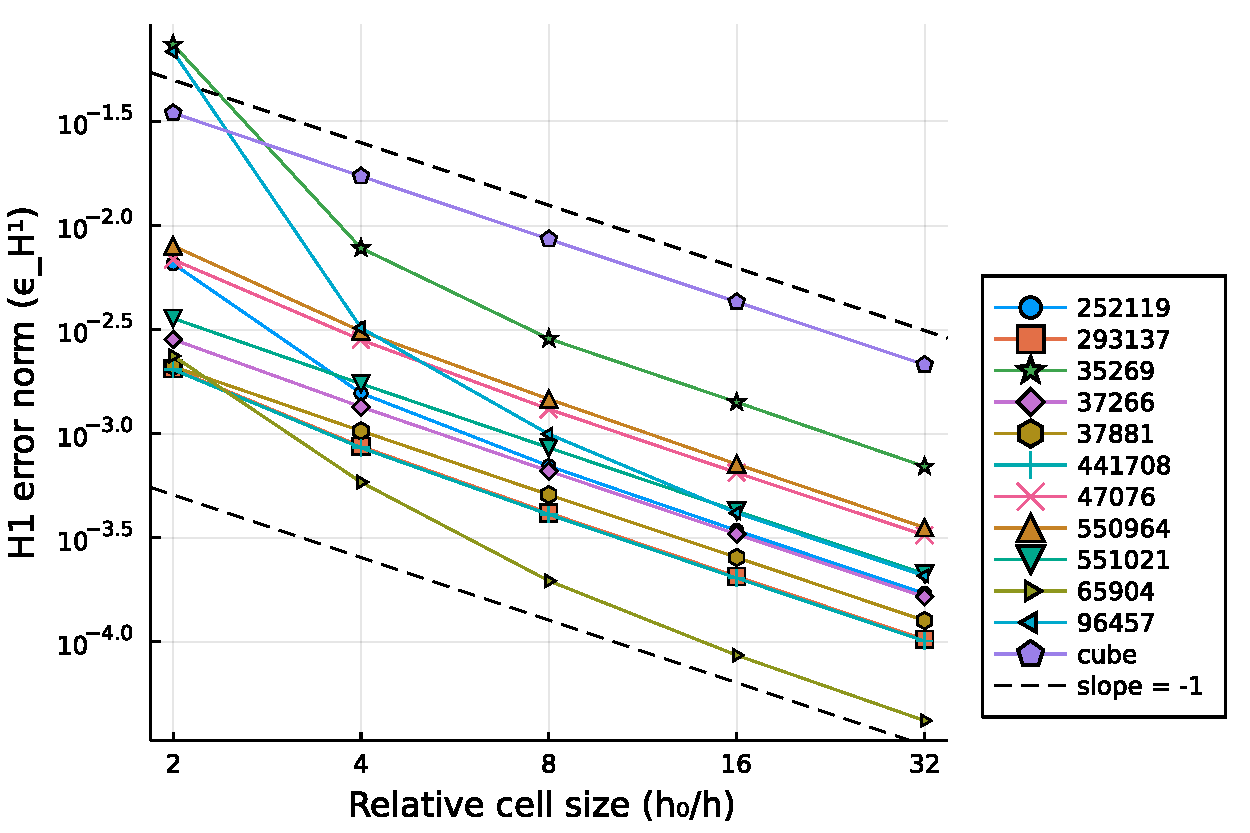
\includegraphics[width=0.49\textwidth]{../analysis/plots/x_nmax_y_error_h1}
  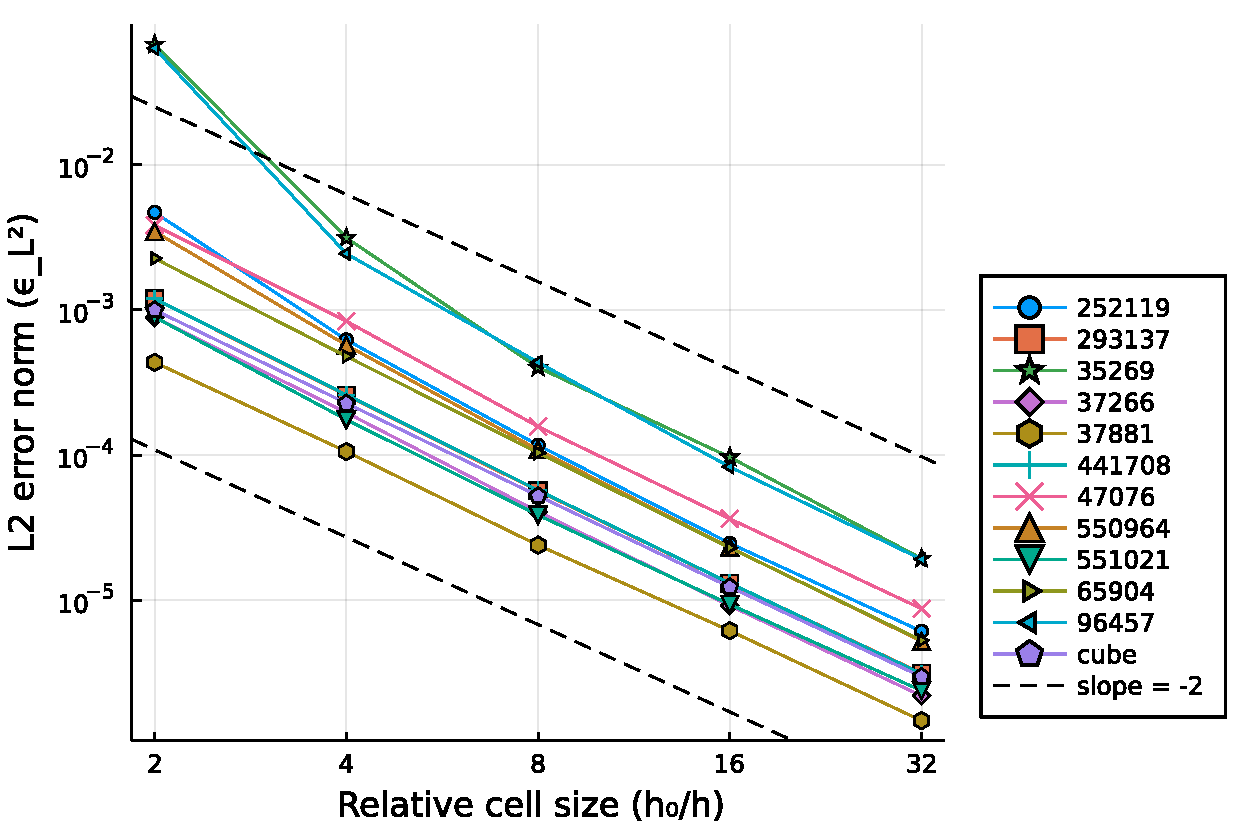
\includegraphics[width=0.49\textwidth]{../analysis/plots/x_nmax_y_error_l2}
\end{frame}

\begin{frame}{3. Large geometry dataset}
  \begin{block}{Setup}
    \begin{itemize}
      \item
        \href{https://ten-thousand-models.appspot.com/results.html?q=is+solid\%2C+is+manifold}
        {\underline{4963 geometries}}
        filtered from \href{https://ten-thousand-models.appspot.com}{Thingi10k}
        (solid and manifold)
      \item
        $N_{max} = 100 $ (unique $h$-refinement criterion)
    \end{itemize}

  \end{block}

  \centering
  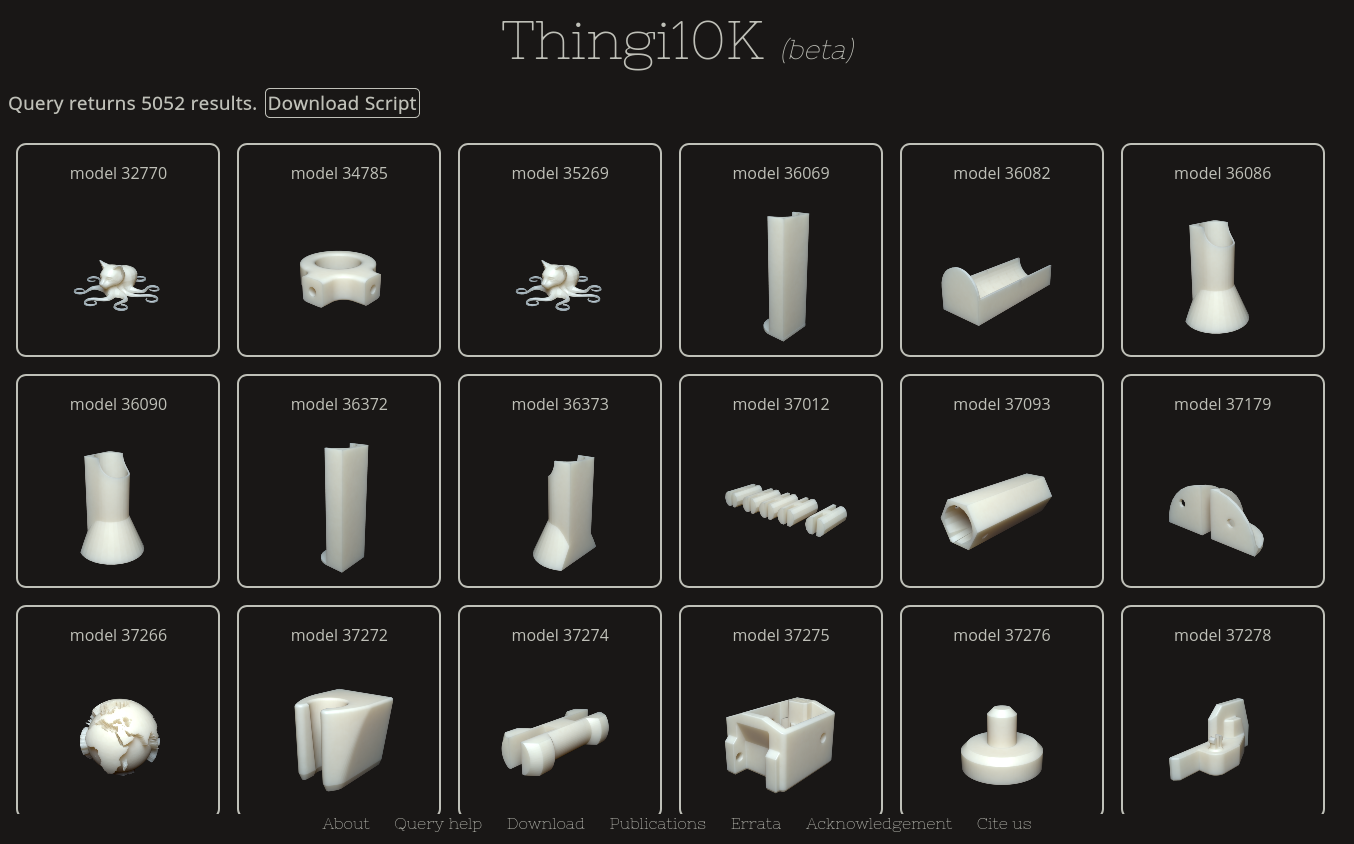
\includegraphics[width=.75\textwidth]{thingi10k_screenshot}
  %% screenshot of thingi10k
\end{frame}

\begin{frame}{3. Large geometry dataset}
  \begin{block}{Summary}
   \dirtree{%
     .1 \textbf{Total}: 4963  .
     .2 Not available: 193 .
     .2 \textbf{Available}: 4770 .
     .3 Ended: 4646.
     .4 \textbf{Success}: 4641.
     .4 Fail: 5.
     .3 Not ended: 124.
     .4 Load error: 5.
     .4 Degenerate 62.
     .4 Too fine: 30.
     .4 Other: 27.
     }

  \end{block}

\end{frame}


\begin{frame}{3. Large geometry dataset}



  \begin{block}{Volume error}
  \begin{itemize}
    \item
      $\epsilon_V = V_{IN} + V_{OUT} - V_{BBOX}$
    \item
      99.9\% of 4641 is below $10^{-10}$
    \item
      Errors related with to deleting small facets properly
  \end{itemize}
  \end{block}

  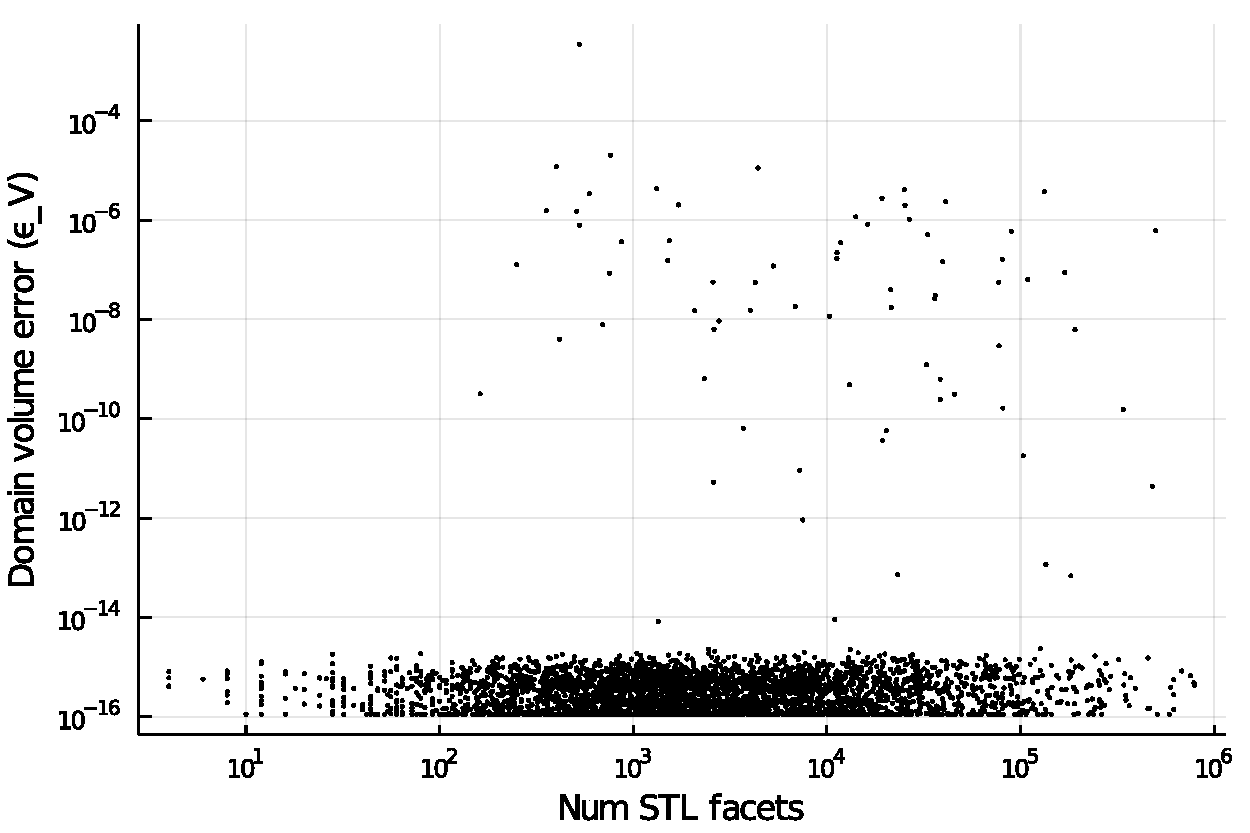
\includegraphics[width=0.49\textwidth]{../analysis/plots/num_stl_facets_volume_error}
  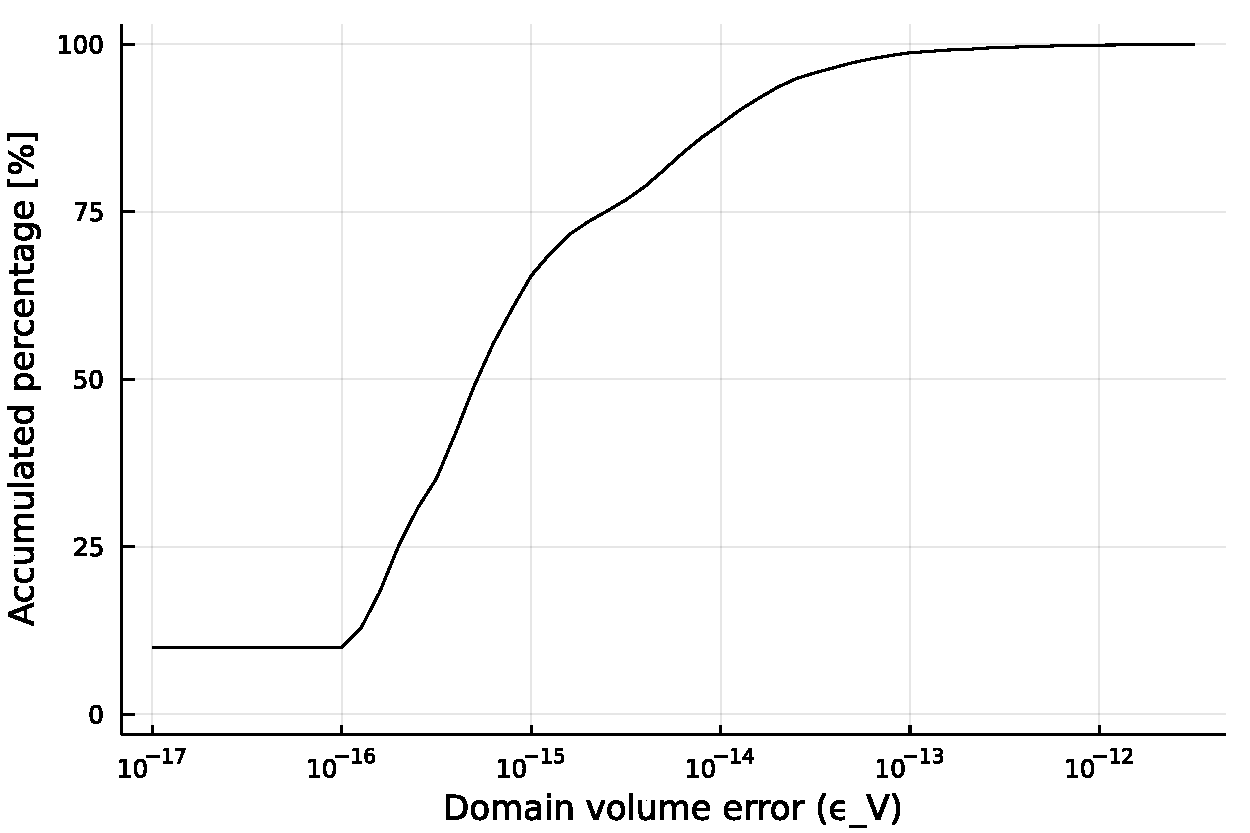
\includegraphics[width=0.49\textwidth]{../analysis/plots/histogram_volume_error}
\end{frame}

\begin{frame}{3. Large geometry dataset}

  \begin{block}{Volume error}
  \begin{itemize}
    \item
      $\epsilon_V = V_{IN} + V_{OUT} - V_{BBOX}$
    \item
      99.9\% of 4641 is below $10^{-10}$
    \item
      Errors related with to deleting small facets properly
  \end{itemize}
  \end{block}

  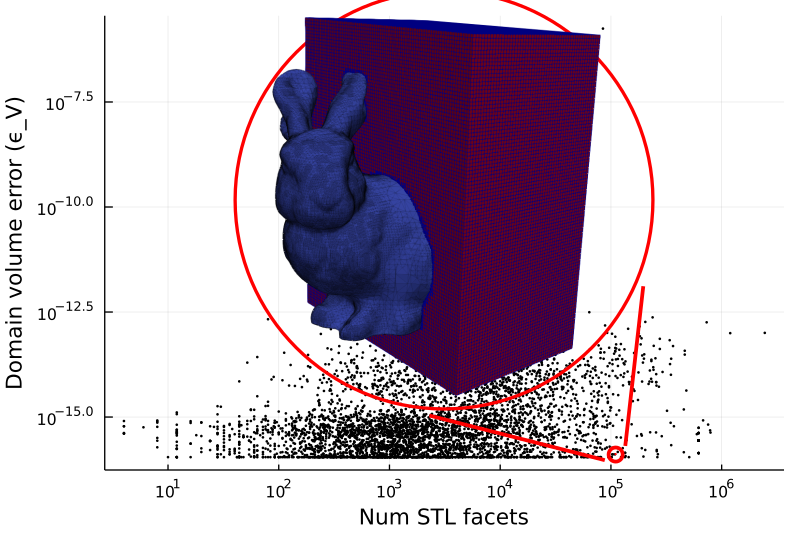
\includegraphics[width=0.49\textwidth]{num_stl_facets_volume_error_bunny}
  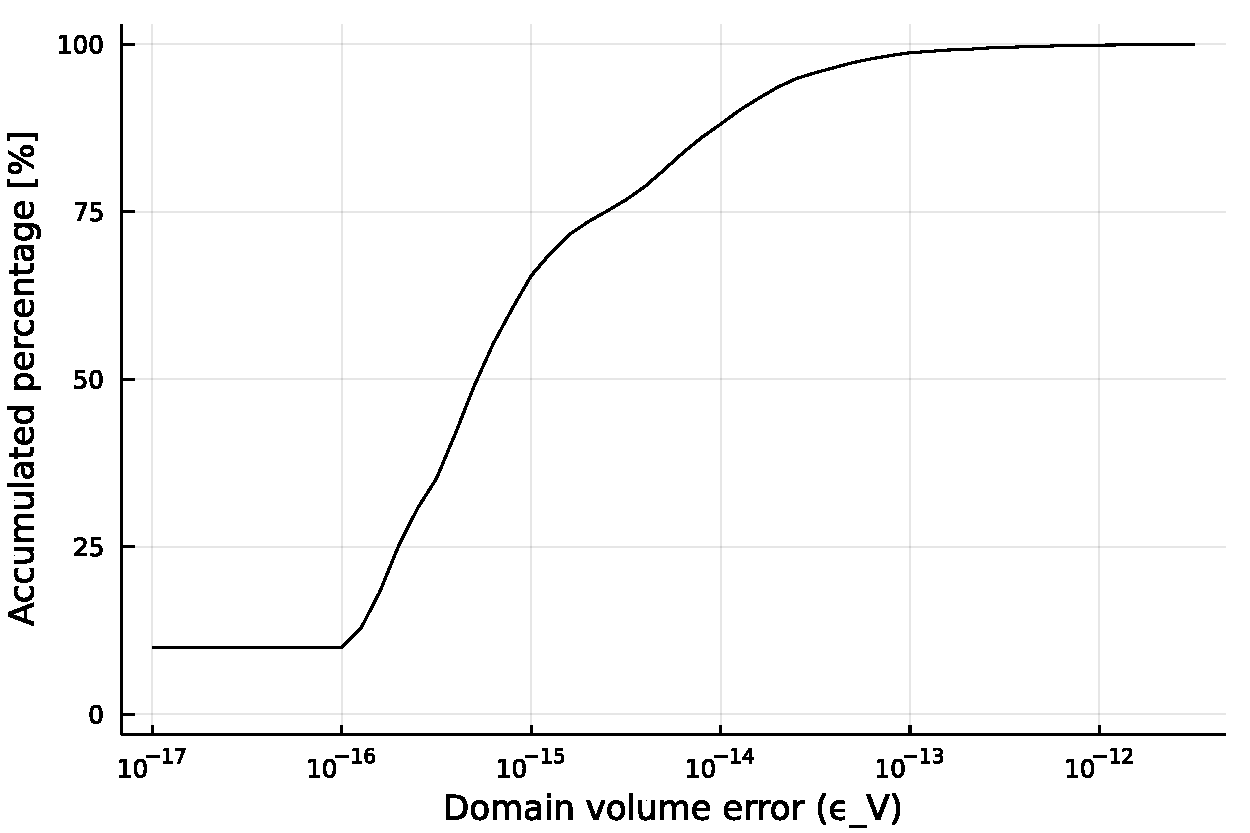
\includegraphics[width=0.49\textwidth]{../analysis/plots/histogram_volume_error}
\end{frame}

\begin{frame}{3. Large geometry dataset}

  \begin{block}{Volume error}
  \begin{itemize}
    \item
      $\epsilon_V = V_{IN} + V_{OUT} - V_{BBOX}$
    \item
      99.9\% of 4641 is below $10^{-10}$
    \item
      Errors related with to deleting small facets properly
  \end{itemize}
  \end{block}

  \includegraphics[width=0.49\textwidth]{num_stl_facets_volume_error_509317}
  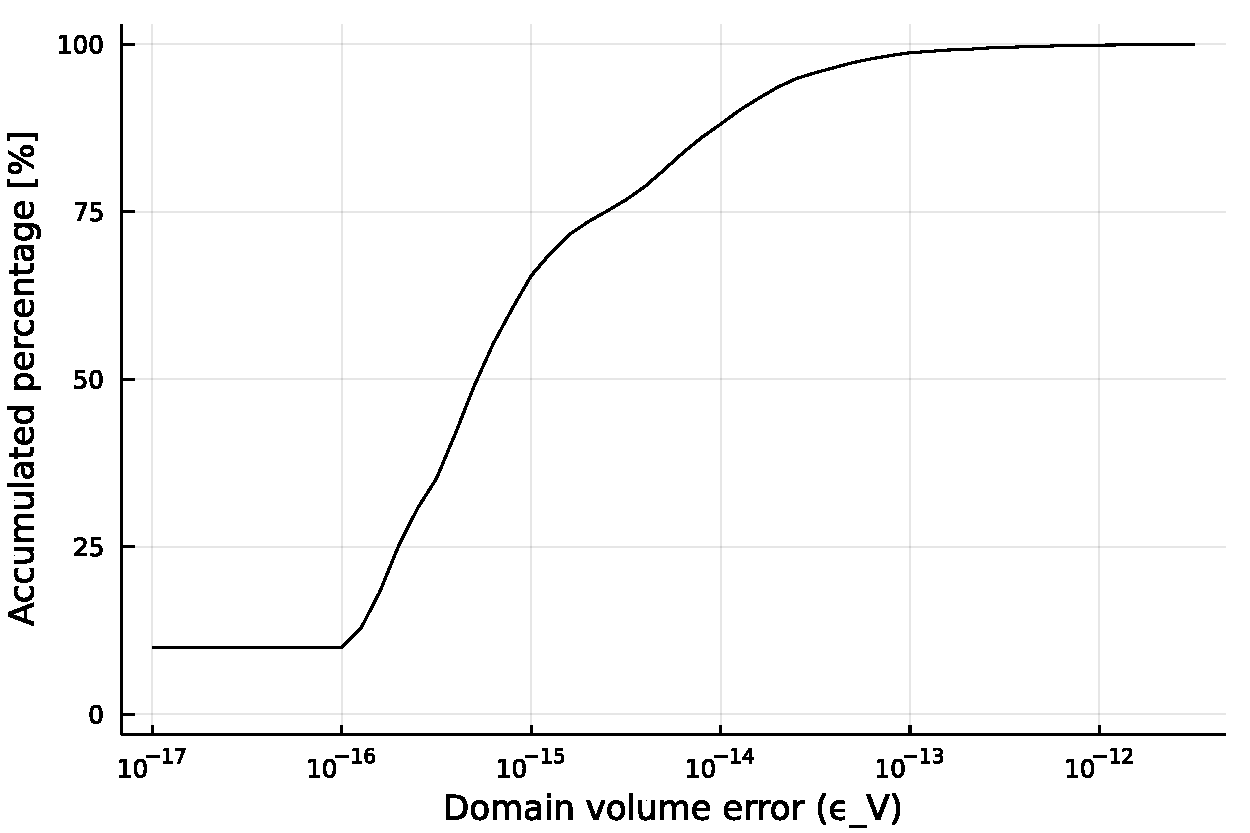
\includegraphics[width=0.49\textwidth]{../analysis/plots/histogram_volume_error}
\end{frame}

%\begin{frame}{3. Large geometry dataset}
%
%  \begin{block}{Volume error [filtering STLs with small facets]}
%  \begin{itemize}
%    \item
%      $\epsilon_V = V_{IN} + V_{OUT} - V_{BBOX}$
%    \item
%      100\% is below $10^{-14}$
%   % \item
%   %   All STLs above $10^{-9}$ contain small facets
%  \end{itemize}
%  \end{block}
%
%  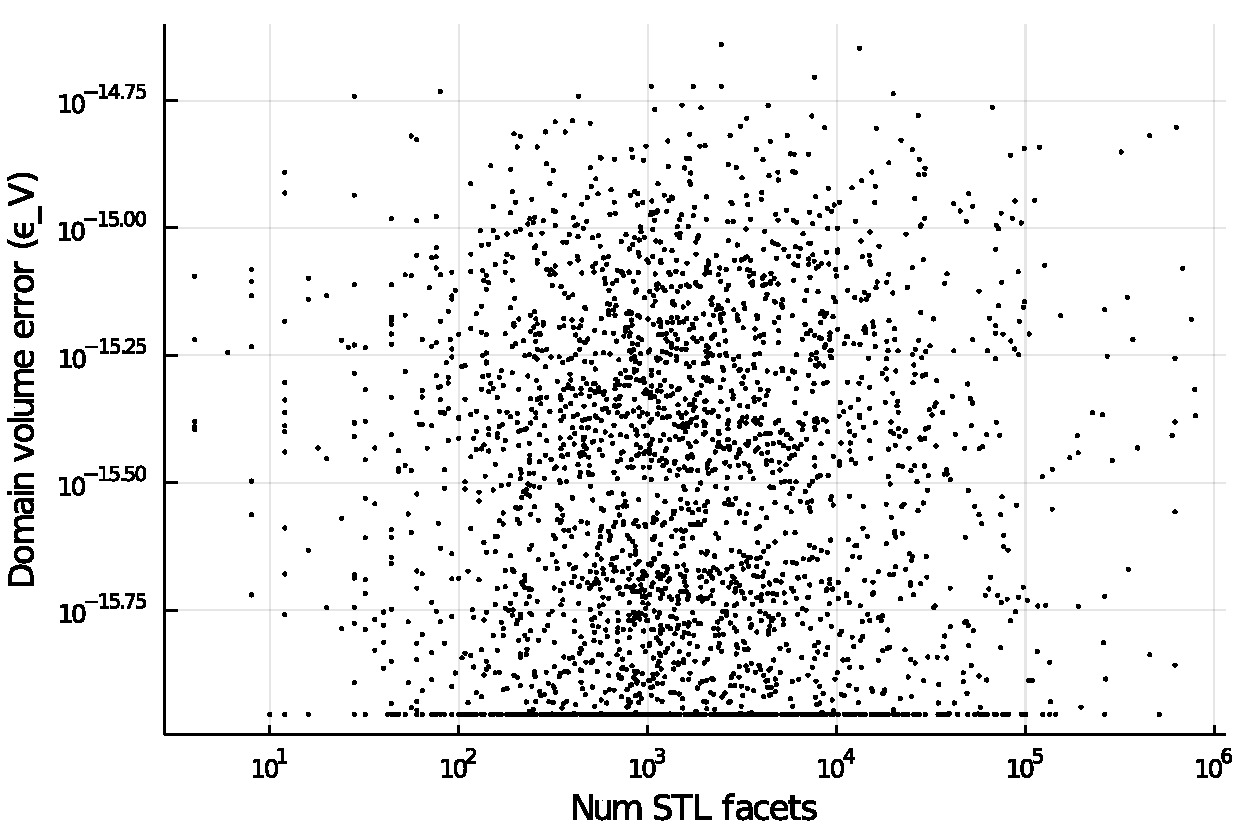
\includegraphics[width=0.49\textwidth]{../analysis/plots/filter_num_stl_facets_volume_error}
%  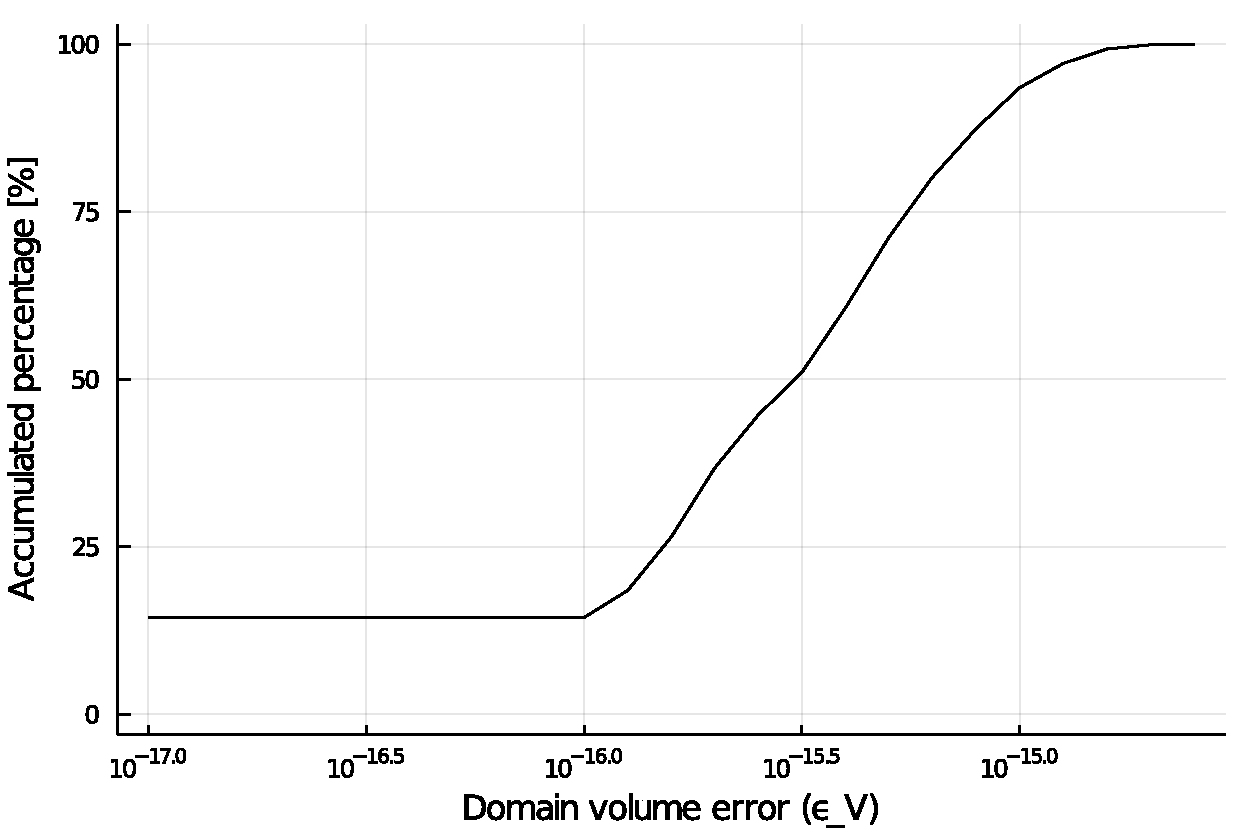
\includegraphics[width=0.49\textwidth]{../analysis/plots/filter_histogram_volume_error}
%\end{frame}

\begin{frame}{3. Large geometry dataset}

  \begin{block}{Surface error}
  \begin{itemize}
    \item
      $\epsilon_\Gamma = \Gamma - V_{STL}$
    \item
      99.9\% of 4641 is below $10^{-9}$
  \end{itemize}
  \end{block}

  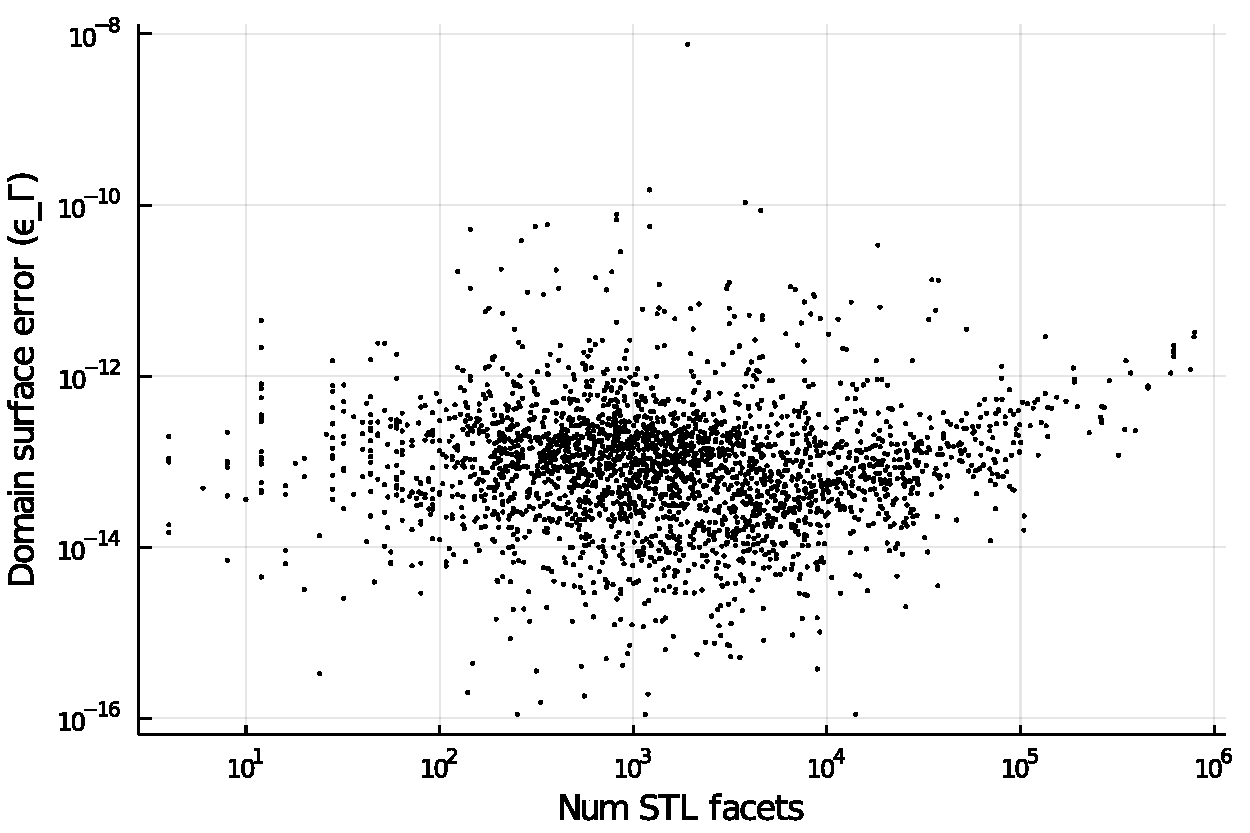
\includegraphics[width=0.49\textwidth]{../analysis/plots/num_stl_facets_surface_error}
  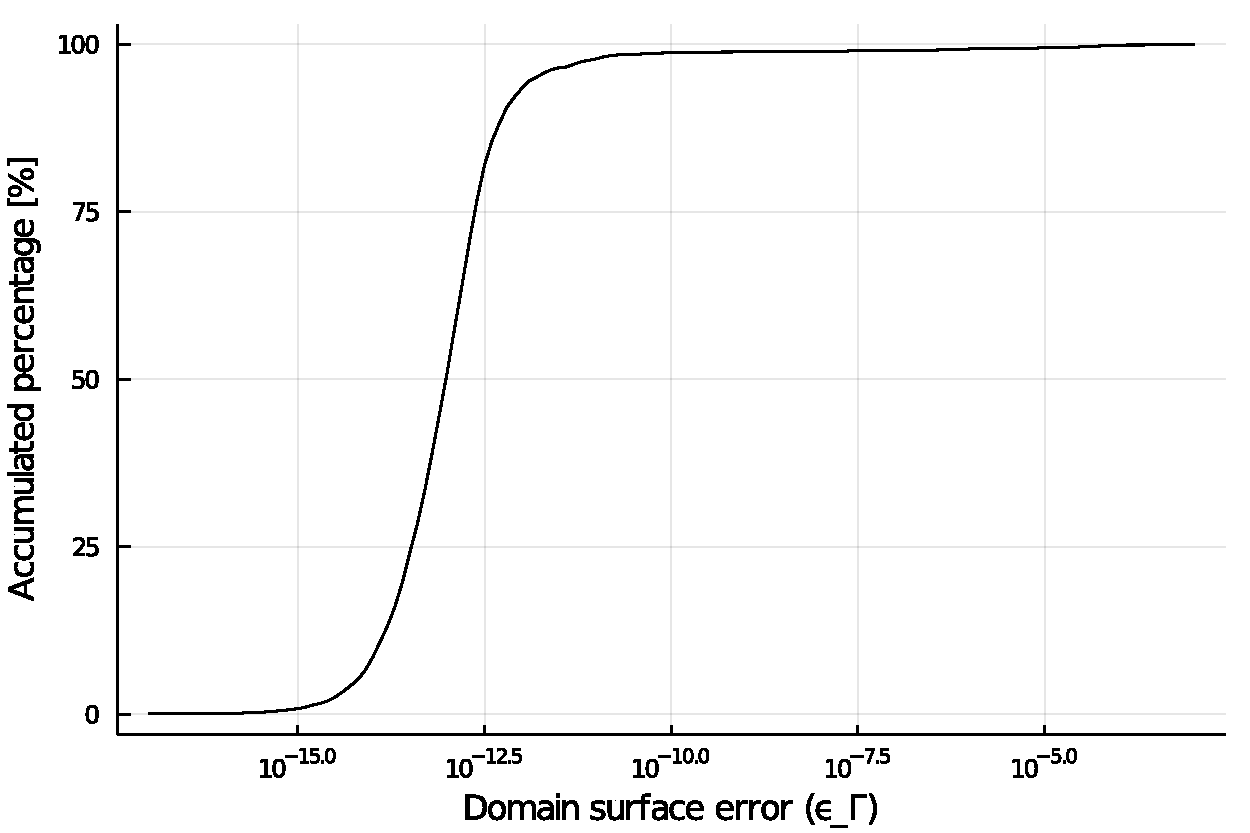
\includegraphics[width=0.49\textwidth]{../analysis/plots/histogram_surface_error}
\end{frame}

%\begin{frame}{3. Large geometry dataset}
%
%  \begin{block}{Surface error [filtering STLs with small facets]}
%  \begin{itemize}
%    \item
%      $\epsilon_\Gamma = \Gamma - V_{STL}$
%    \item
%      99.9\% is below $10^{-9}$
%    \item
%      One outlier can be moved by increasing the tolerance
%  \end{itemize}
%  \end{block}
%
%  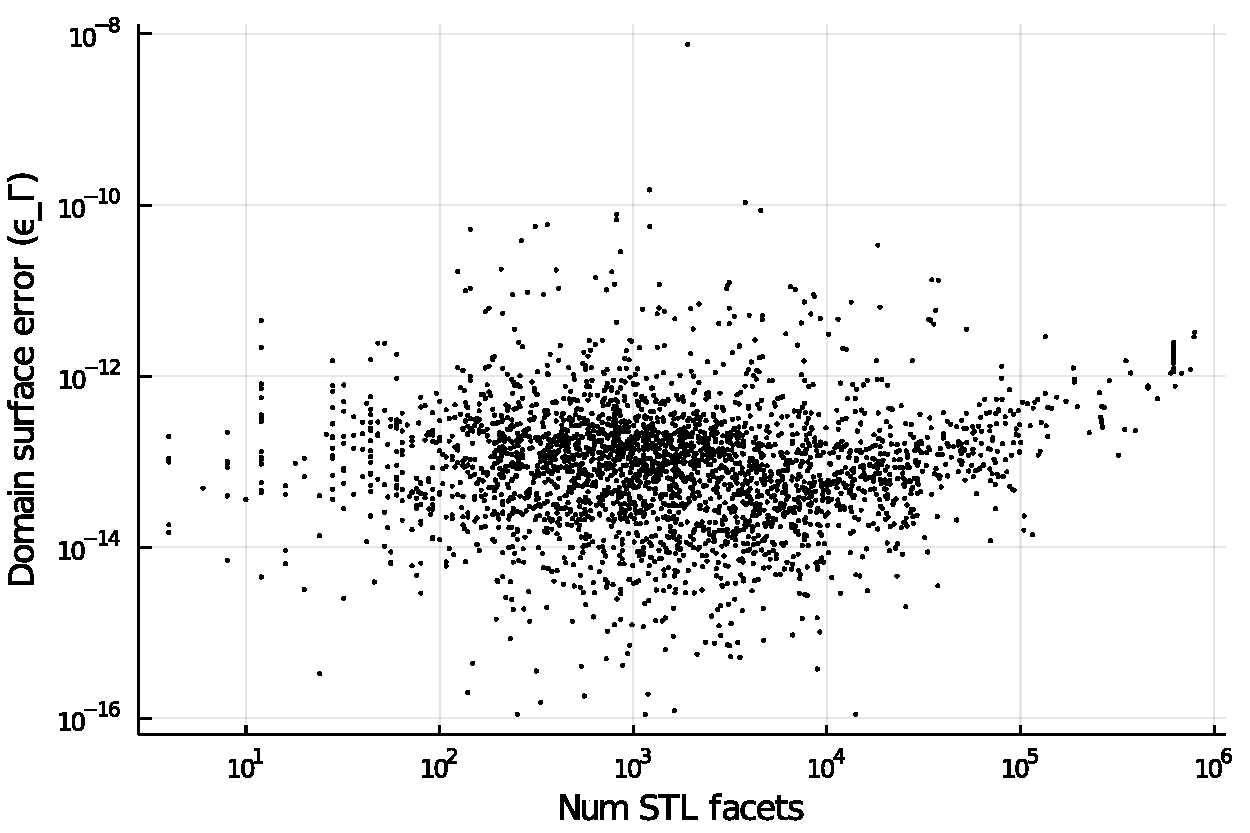
\includegraphics[width=0.49\textwidth]{../analysis/plots/filter_num_stl_facets_surface_error}
%  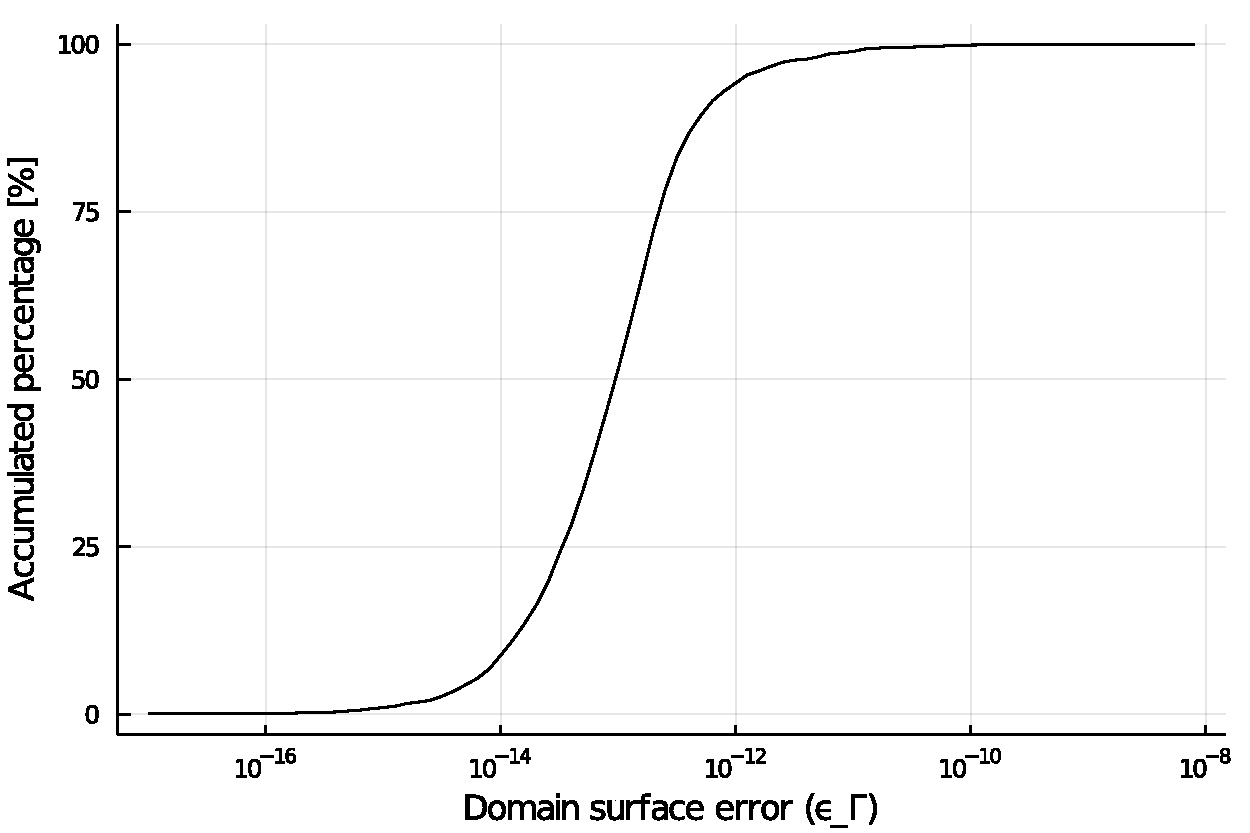
\includegraphics[width=0.49\textwidth]{../analysis/plots/filter_histogram_surface_error}
%\end{frame}
%
%\begin{frame}{3. Large geometry dataset}
%
%  \begin{block}{Surface error [filtering STLs with small facets]}
%  \begin{itemize}
%    \item
%      $\epsilon_\Gamma = \Gamma - V_{STL}$
%    \item
%      99.9\% is below $10^{-9}$
%    \item
%      One outlier can be moved by increasing the tolerance
%  \end{itemize}
%  \end{block}
%
%  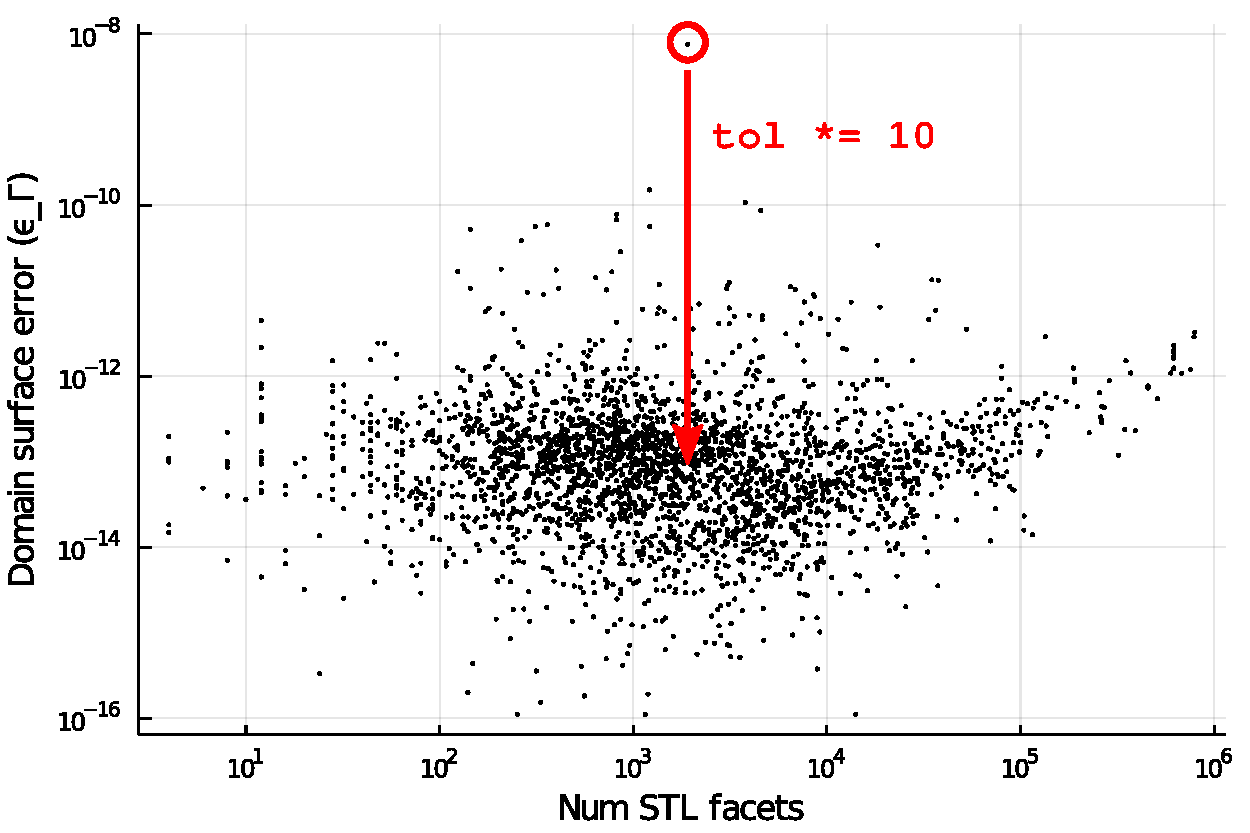
\includegraphics[width=0.49\textwidth]{moving_filter_num_stl_facets_surface_error}
%  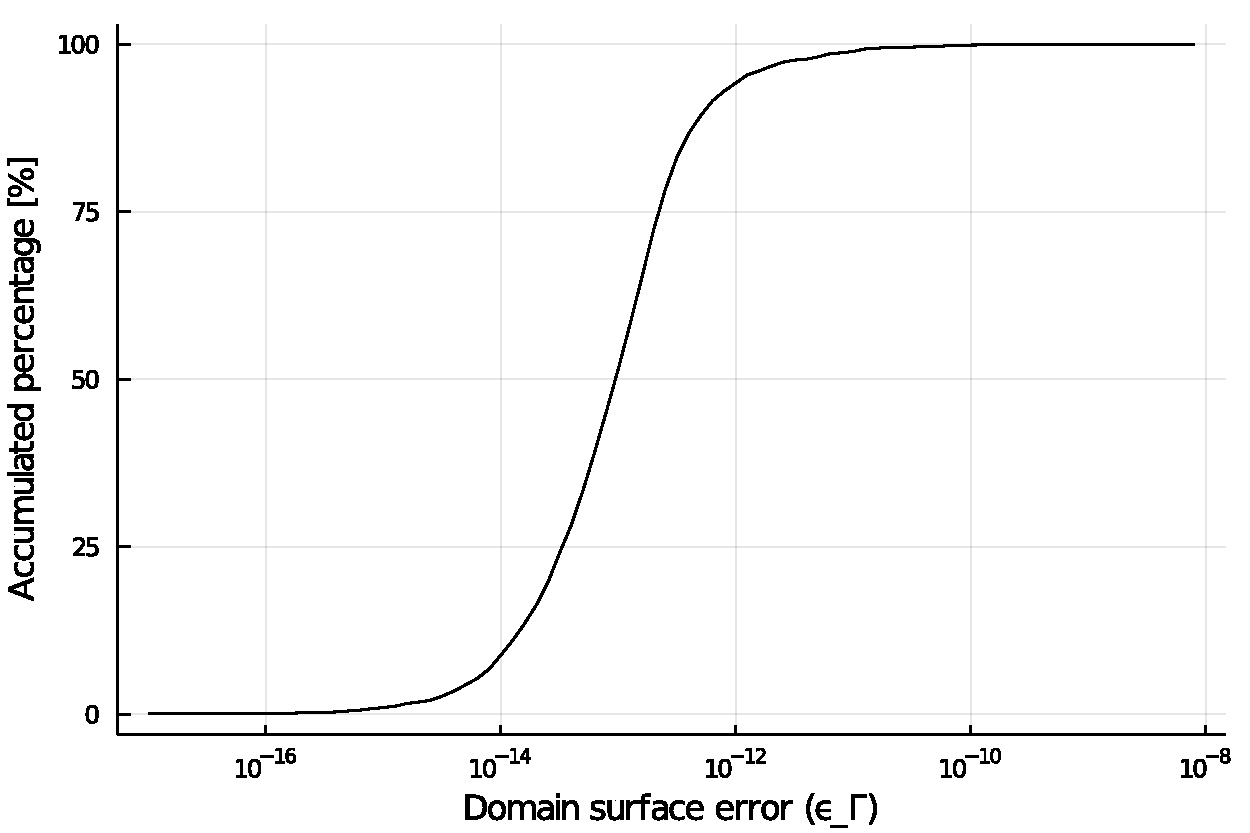
\includegraphics[width=0.49\textwidth]{../analysis/plots/filter_histogram_surface_error}
%\end{frame}

\begin{frame}{3. Large geometry dataset}

  \begin{block}{CPU time}
  \begin{itemize}
    \item
      Not precise measure (different machines, single runs, single cpu)
    \item
      Increasing with the number of STL facets
    \item
      Some geometries have been run with multi-threading and optimized code but discarted in this plot to avoid noise
  \end{itemize}
  \end{block}

  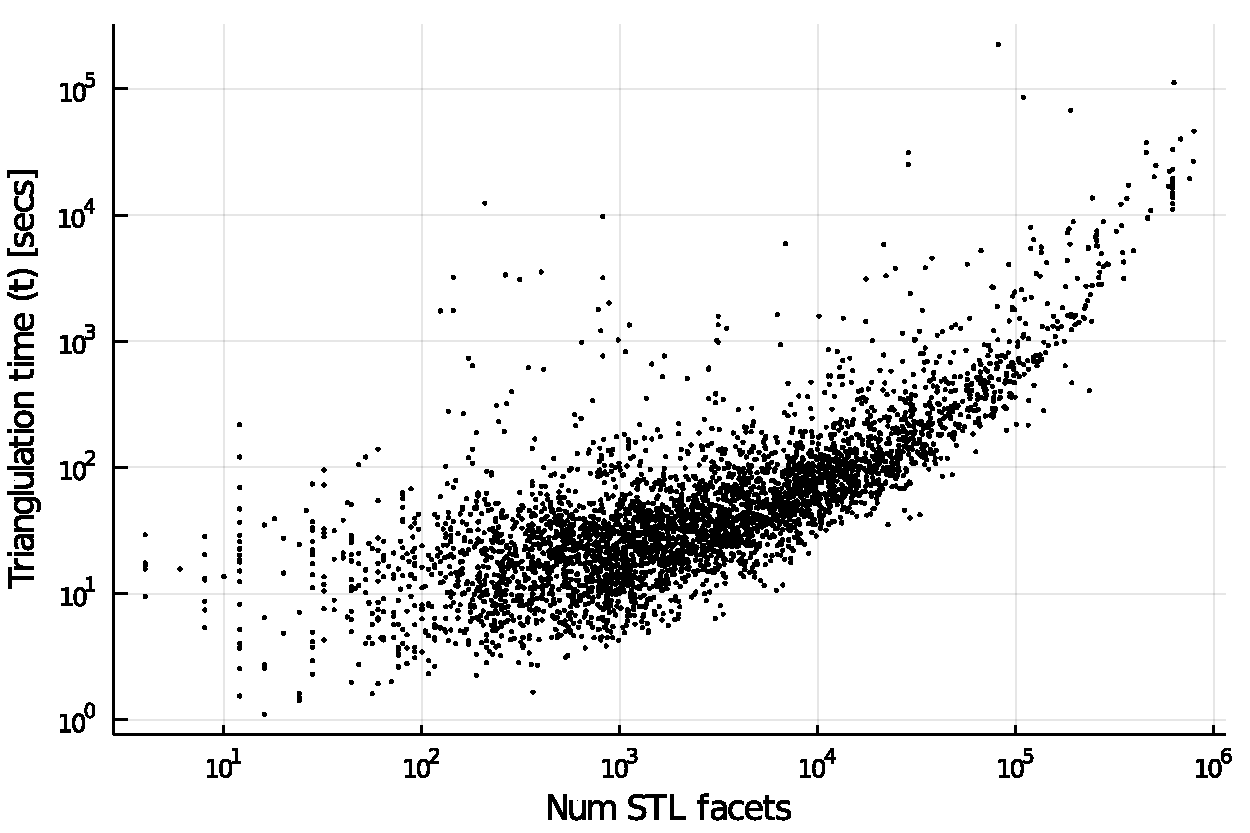
\includegraphics[width=0.49\textwidth]{../analysis/plots/num_stl_facets_time}
  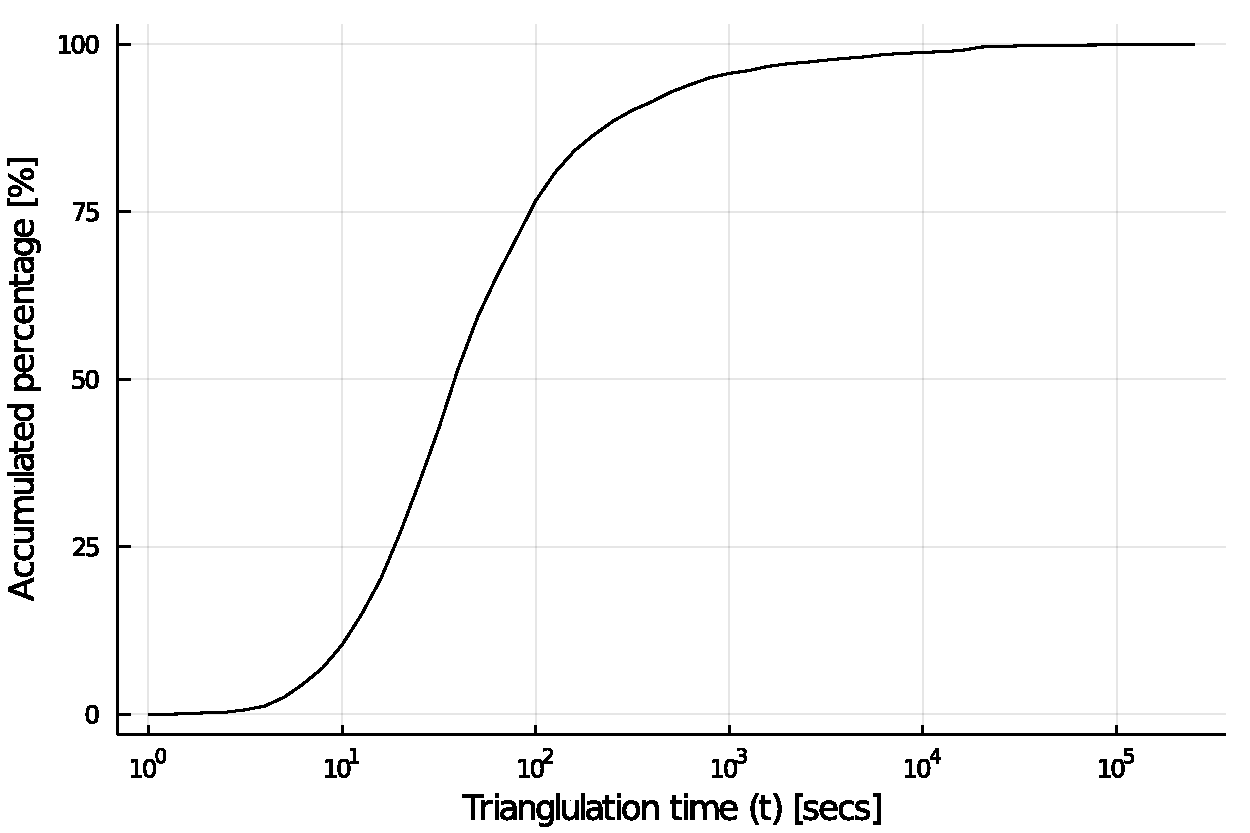
\includegraphics[width=0.49\textwidth]{../analysis/plots/histogram_time}
\end{frame}

\begin{frame}{Conclusions and pending work}

  \textbf{Conclusion so far}
  \begin{itemize}
    \item
      Issues are depending on the geometry
    \item
      Most of problematic geometries can be found \textit{a priori}
    \item
      Optimal convergence with AgFEM
  \end{itemize}
  \textbf{Ongoing work}
  \begin{itemize}
    \item
      Detect true degenerated geometries
  \end{itemize}


\end{frame}
\end{document}
